\renewcommand{\thechapter}{4}

\chapter{Calibrating the Combined Energy Scale}
\label{Ch:E_Scale_Cal}

This section outlines the method used to calibrate the energy scale of the LUX detector for electronic recoils. The idea behind the method is to take calibration data with multiple sources and/or electric fields then combine the measured scintillation signals, primary (S1) and secondary (S2) in order to reconstruct energy. For a given energy deposit in liquid xenon an amount of quanta released is proportional to a work function W, for nuclear recoils we must also consider heat loss. The quanta created at the interaction site are the results of electron-ion pairs and excitons produced by the recoiling xenon nucleus that become photons and electrons, equation \ref{eq:E_Q_ER}.
\begin{equation}
\begin{split}
\rm E= W (n_i + n_{ex}) \\
\rm E= W (n_\gamma + n_e)  \\
\label{eq:E_Q_ER}
\end{split}
\end{equation}

\noindent where E is the energy of the deposition in keV, $\rm n_i$, $\rm n_{ex}$, $\rm n_\gamma$ and $\rm n_e$ are the number of ions, excitons, photons and electrons respectively. The work function (W) for xenon has been measured to be 13.7 $\rm \pm$ 0.2  eV/quanta  \cite{Dahl_Thesis}.
Excitons quickly de-excite and contribute to the primary scintillation signal (S1). Ions that recombine with their electron pairs produce scintillation light (S1), while those electrons that do not recombine are collected several $\rm \mu s$ later in the extraction region as the larger secondary scintillation signal S2. The interactions of NR and ER type events were discussed previously in \ref{sec:LXe_Theory}.


There are two knobs to turn that tune the recombination fraction and probe combined energy space over a variety of S1 and S2, we can either change the energy of the source or adjust the drift field. The larger the spread in S1 and S2 the more constrained the combined energy scale will be. Measuring both light and charge allows for a vastly improved resolution compared with only using a single S1 or S2 only space, since recombination fluctuations cancel out if energy is reconstructed correctly. Using equation \ref{eq:E_Q_ER} and assuming that the heat loss is negligible for electronic recoils (ER) we can reconstruct energy by knowing the work function and the conversion from measured S1(light) and S2(charge) signals to the number of quanta ($\rm n_\gamma + n_e$) liberated by the interaction. We define gain-1 (g1) and gain-2 (g2) as the conversion from the average number of photons and electrons propagated from the interaction site to the observed signal by the PMT arrays as a photo electron (PE), given in equation \ref{eq:Gain1}. Note for the value of S2 in this section we only use the signal on the bottom PMT array $\rm S2_b$.
\begin{equation}
\begin{split}
\rm  \left<n_\gamma\right> = \frac{\left<S1\right>}{g_1}\\
\rm \left<n_{e}\right> = \frac{\left<S2\right>}{g_2}
\label{eq:Gain1}
\end{split}
\end{equation}

\noindent By using multiple mono energetic sources with known energies we can extract a best fit for the value of the gains (g1,g2) by making a Doke plot \cite{Doke_alpha} \cite{alpha_xenon}. The mono energetic lines used for the purposes of the calibration are listed in table \ref{table:Cal_lines}. For each calibration point we calculate the mean light yield and charge yield and fit a line, S1/E and S2/E respectively, (Equation \ref{eq:Doke}).
\begin{equation}
\begin{split}
\rm  S1/E= \frac{n_\gamma}{(n_\gamma+n_e)}\times\frac{g1}{W} \\
\rm  S2/E= \frac{n_e}{(n_\gamma+n_e)}\times\frac{g2}{W}
\label{eq:Doke}
\end{split}
\end{equation}

\noindent Fitting equation \ref{eq:Doke} to a line yields

\begin{equation}
\begin{split}
%\rm  1= \left(\frac{S1}{E}\right)\left(\frac{W}{g1}\right) + \left(\frac{S2}{E}\right)\left(\frac{W}{g2}\right) \\[0.5ex]
\rm  \left(\frac{S1}{E}\right)=\left(\frac{g1}{W}\right) - \left(\frac{S2}{E}\right)\left(\frac{g1}{g2}\right) \\
\rm y=\frac{S1}{E}, x=\frac{S2}{E} \\
\rm y= m\cdot x + b
%\rm g1=b\cdot W \\
%\rm g2=\frac{g1}{m}=\frac{b\cdot W}{m}
\label{eq:LinFit}
\end{split}
\end{equation}

\noindent The x and y intercepts from Equation \ref{eq:LinFit} can be used to solve for g1 and g2. 

\begin{equation}
\begin{split}
%\rm  1= \left(\frac{S1}{E}\right)\left(\frac{W}{g1}\right) + \left(\frac{S2}{E}\right)\left(\frac{W}{g2}\right) \\[0.5ex]
%\rm  \left(\frac{S1}{E}\right)=\left(\frac{g1}{W}\right) - \left(\frac{S2}{E}\right)\left(\frac{g1}{g2}\right) \\
%\rm y=\frac{S1}{E}, x=\frac{S2}{E}, y= m\cdot x + b \\
\rm g1=b\cdot W \\
\rm g2=\frac{g1}{m}=\frac{b\cdot W}{m}
\label{eq:g1g2_linfit}
\end{split}
\end{equation}


The values of g1,g2 are degenerate and highly correlated such that the ratio of g1:g2 is always a constant, a reduction in g1 can be compensated by an increase in g2 and still yield the same number of initial quanta and visa versa. Breaking the degeneracy requires data over a wide range of S1 and S2 values near the intercept of the Doke plot. Due to the strong correlation in the fit parameters the data is fit by minimizing the likelihood and the errors in intercept and slope are determined using MCMC (Markov Chain Monte Carlo). 




\begin{table}[h!]
%\caption{Nonlinear Model Results}
\centering
\footnotesize
\begin{tabular}{|c|c|c|}
\hline
Source & Energy [keV] &Decay Type  \\ [0.5ex] % inserts table %heading
\hline
Xe K shell  & 29.7, 34 	 		& X-ray							\\ \hline
 $\rm ^{83m}Kr$ 	& 41.55**		& Internal Conversion			\\ \hline
 $\rm ^{131}Xe$ 	& 163.9		& Internal Conversion			\\ \hline
$\rm ^{127}Xe$ 	& 203 or 375	& $\rm^{127}$I daughter $\rm \gamma$-emission	\\ \hline
				      & 33.8			& Kb shell X-ray 						\\ \hline
				      & 5.3			& L shell X-ray 					\\ \hline
$\rm ^{129m}Xe$	& 236.1		& Internal Conversion 			\\ \hline
$\rm ^{214}Bi	$	& 609 			& $\rm \gamma$-emission				 \\ \hline
 $\rm ^{137}Cs$	& 661.6		& Photo-absorption 					\\ [0.5ex] 
\hline
\end{tabular}
\caption{Mono energetic peaks used for g1 g2 calibration. ** $\rm^{83m}Kr$ data was taken at 50 and 100 [V/cm] along with the standard field of 170 [V/cm].}
\label{table:Cal_lines}
\end{table}



\section{Anti-Correlation Space}
The first step in calibrating the energy scale is to plot the observables S1 vs. S2, by doing this the anti correlation between light and change at a given energy become apparent, figure \ref{fig:S1S2_space}. For the data presented here a fiducial cut was placed at a radius of less than 18 [cm] and drift distance between 6 and 46 [cm] which greatly reduces the background event rate. To extract g1 g2 we first determine the average values of S1 and S2 at each known energy. Initially loose diagonal cuts are placed by eye on the populations, figure \ref{fig:S1S2_space}. Next, using a un-binned maximum likelihood fit the mean and sigma are estimated and then refit using $\rm \pm 2\sigma$ of the initial distribution to remove tails from backgrounds. With the initial estimate for the mean S1 and S2 response to a given energy the gains g1,g2 are determined. The resulting value of g1 and g2 is found to be 0.096 $\pm$ 0.009 and 5.94 $\pm$ 1.68 respectively, the fit is shown in figure \ref{fig:Doke1}. The values of g1 and g2 represent a best fit tot he underling recombination theory where for each additional photon there is a corresponding reduction of one electron and visa versa. The method for extracting the uncertainties using MCMC will be discussed later in section \ref{sec:MCMC}.

\begin{figure}[h!]\centering
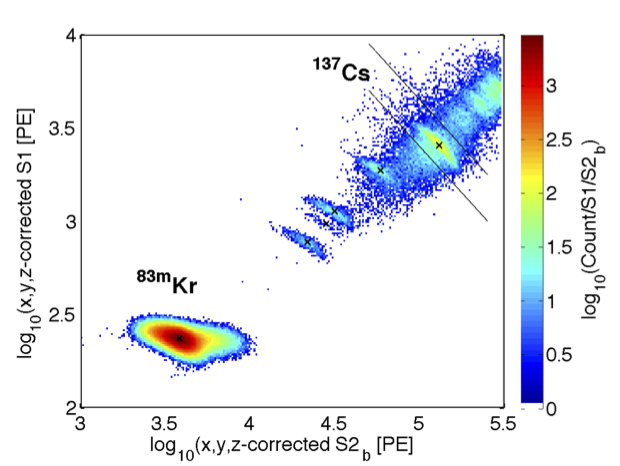
\includegraphics[width=70mm]{Chapter_E_Scale/Figures/S1S2_density_Kr_Cs_fit.png}
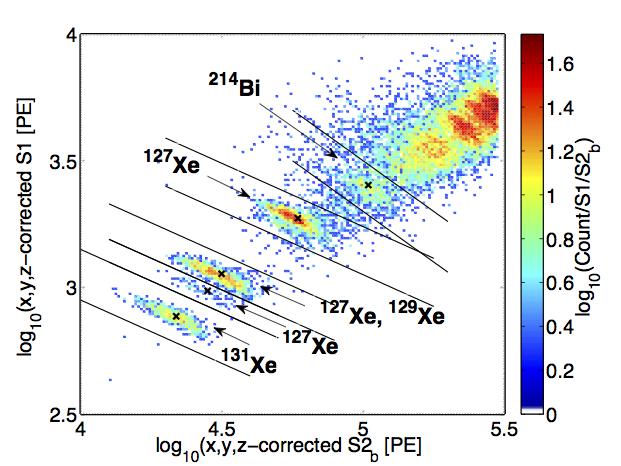
\includegraphics[width=70mm]{Chapter_E_Scale/Figures/S1S2_density_XeA_fit.png}
\caption{LUX data in anti correlation space (S1 vs. S2), the black lines indicate the initial cuts by eye used to isolate populations of constant energy. In both figures diagonals represent lines of constant energy with a slope depending on the local recombination probability. The centroids found by an unbind maximum likelihood analysis are shows as a black X, for sources show in table \ref{table:Cal_lines}. }
\label{fig:S1S2_space}
\end{figure}

 \begin{figure}[h!]\centering
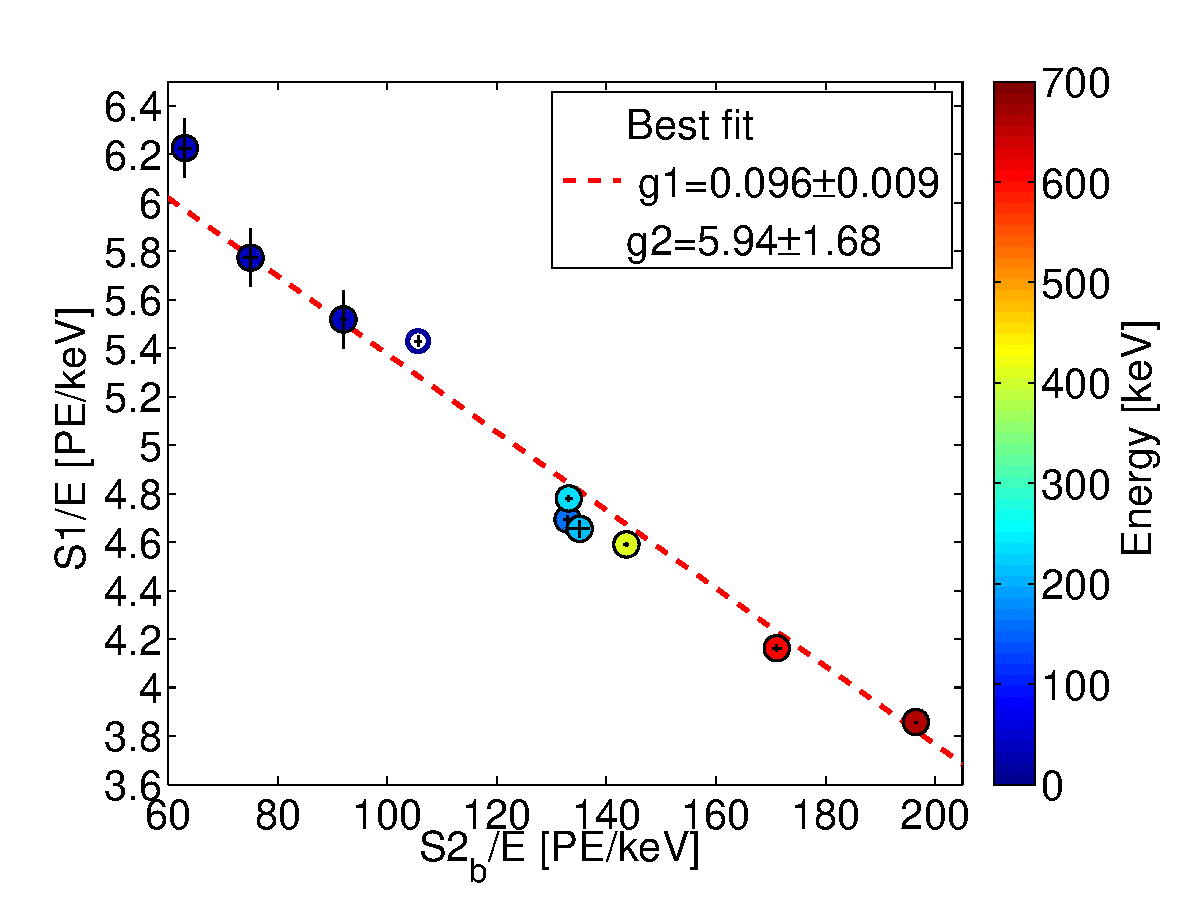
\includegraphics[width=120mm]{Chapter_E_Scale/Figures/S1S2_Doke_1.eps}
\caption{Doke plot showing the best fit for the energy calibration parameters g1 and g2 using S1 and S2 means extracted from anti-correlation space. The first three blue points, from the left, are from $\rm^{83}Kr$ calibrations at 50, 100 and 170 V/cm respectively. The open circle was from the K-shell xenon X-ray and was not used for the fit as it's absolute energy and origin from the skin of the detector is uncertain.}
\label{fig:Doke1}
\end{figure}

\section{Refitting in Combined Energy Space}
From the first attempt to find g1,g2 in figure \ref{fig:Doke1} there are discrepancies between the data and the fit, however this first result is only a crude estimate derived from anti correlation space. Once we have an initial estimate of gains g1,g2 a combined energy scale can be constructed with significantly improved resolution over the initial guess, due to the fact that recombination fluctuations are canceled. With the improved resolution the data are fit around the combined energy peaks using an unbinned maximum likelihood fit to a normal distribution, and then the data refitted around 1.5 $\sigma$ of the initial fit. The fits used to extract the means and sigmas  of the S1 and S2 signals at a given energy are show in figures \ref{fig:Doke_Fits_S1} and \ref{fig:Doke_Fits_S2}. We iterate this technique twice as the convergence is rapid, in this case the initial value of g1 and g2 derived from anti-correlation space are already a close approximation to the true value. The resulting value of g1 and g2 is found to be 0.097$\pm$0.008 and 5.75$\pm$1.4 respectively, the fit is shown in figure \ref{fig:Doke2}. After refitting there is a significant improvement over figure \ref{fig:Doke1}, especially the xenon activation lines in the center, which is due to better peak finding in combined energy space over anti-correlation space.


\begin{equation}
\begin{split}
\rm  g1 = 0.097\pm0.008 \\
\rm  g2= 5.75\pm1.4
\label{eq:g1g2Fit}
\end{split}
\end{equation}


 \begin{figure}[h!]\centering
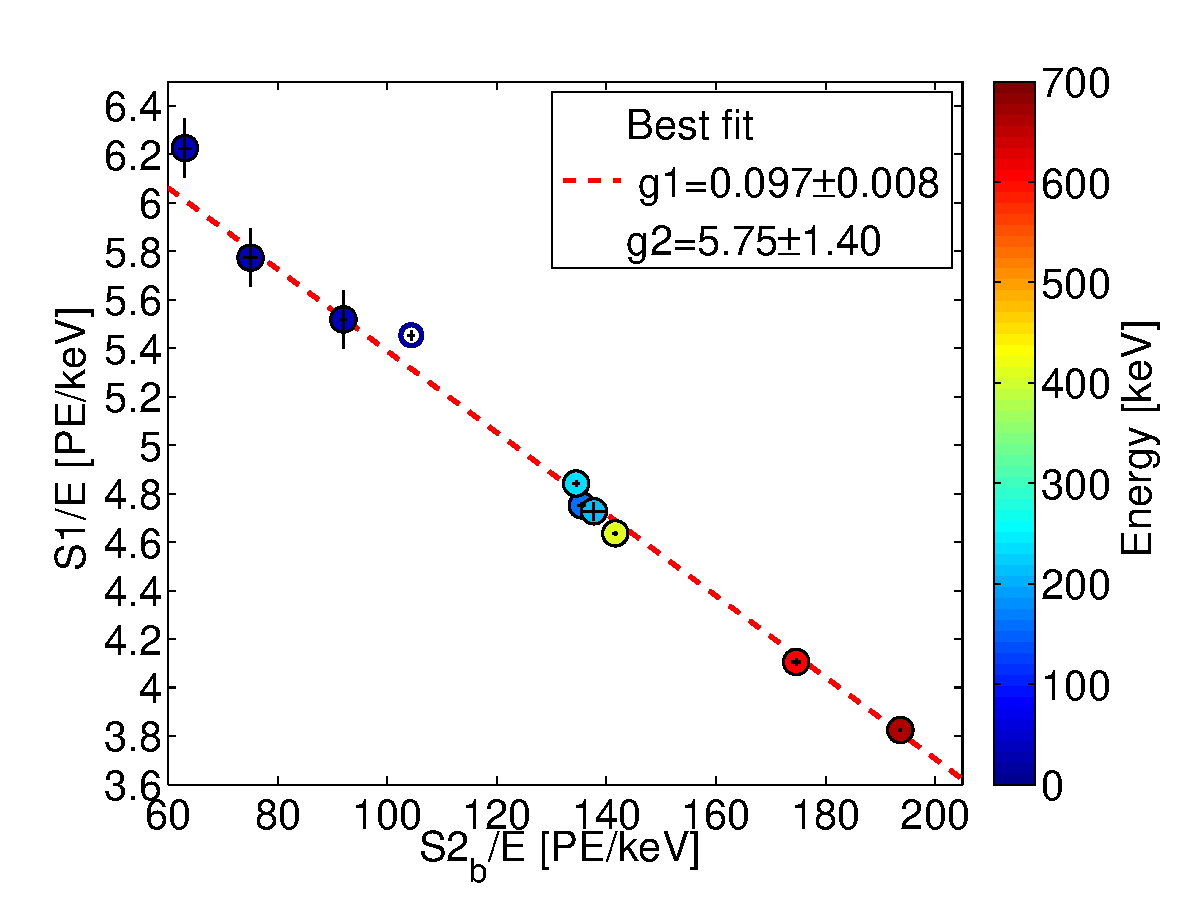
\includegraphics[width=120mm]{Chapter_E_Scale/Figures/S1S2_Doke_3.eps}
\caption{Doke plot showing the best fit for the energy calibration parameters g1 and g2 using S1 and S2 extracted from a combined energy space. The first three blue points, from the left, are from $\rm^{83}Kr$ calibrations at 50, 100 and 170 V/cm respectively. The open circle was from the K-shell xenon X-ray and was not used for the fit as it's absolute energy and origin from the skin of the detector is uncertain.}
\label{fig:Doke2}
\end{figure}

 \begin{figure}[h!]\centering
 
\subcaptionbox{\label{fig:1a}}{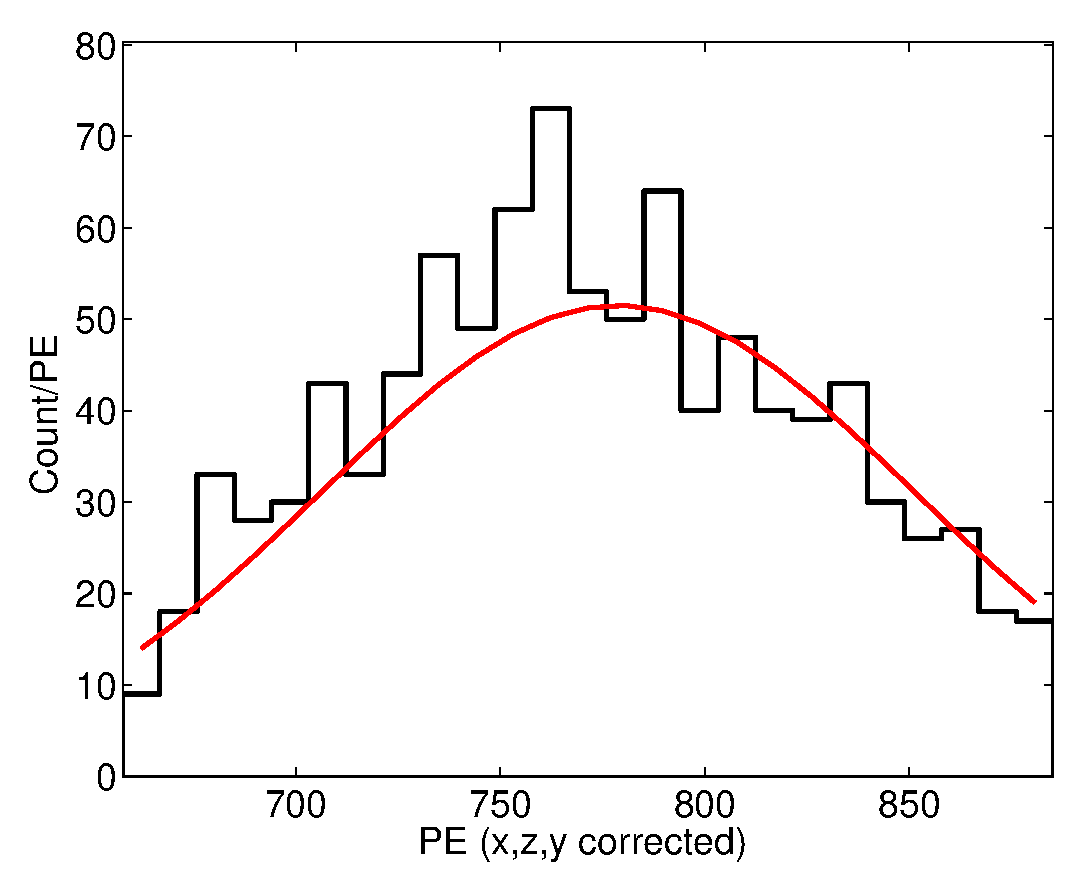
\includegraphics[width=45mm]{Chapter_E_Scale/Figures/Doke_Fits/fit_S1_163.eps}}
\hfill
\subcaptionbox{\label{fig:1b}}{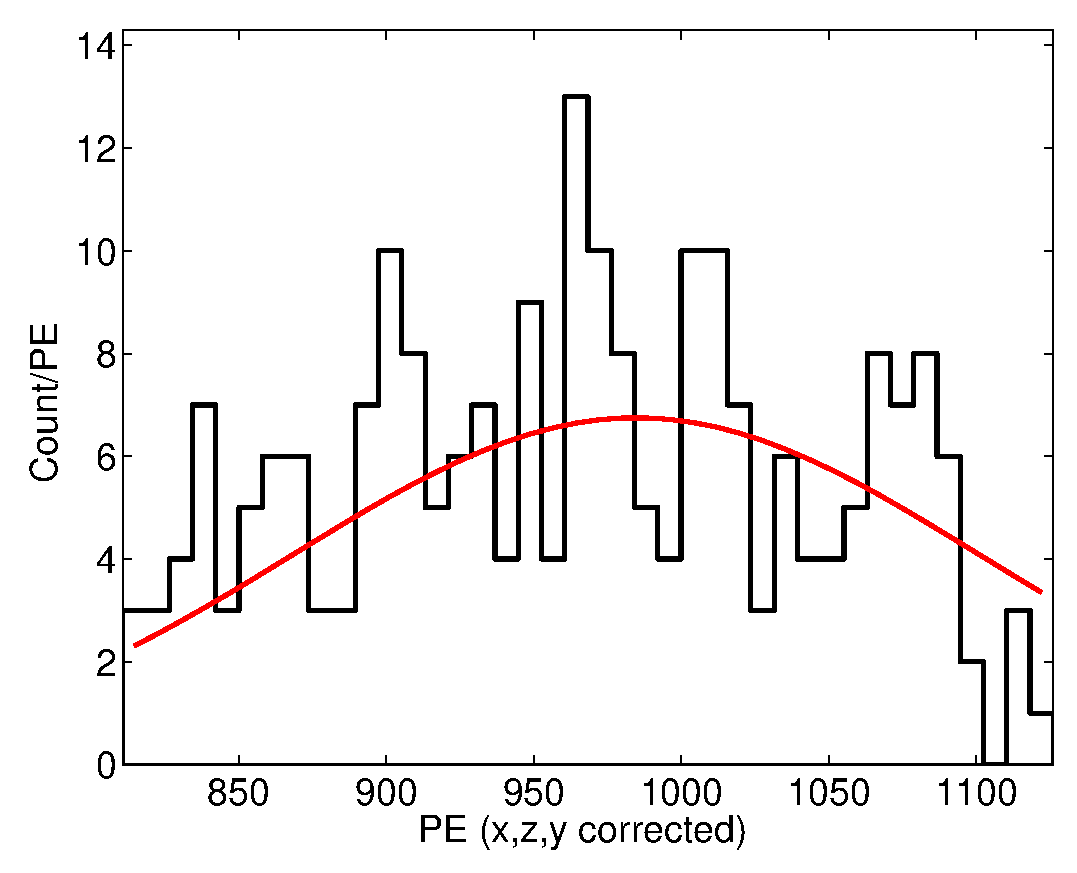
\includegraphics[width=45mm]{Chapter_E_Scale/Figures/Doke_Fits/fit_S1_207.eps}}
\hfill
\subcaptionbox{\label{fig:1c}}{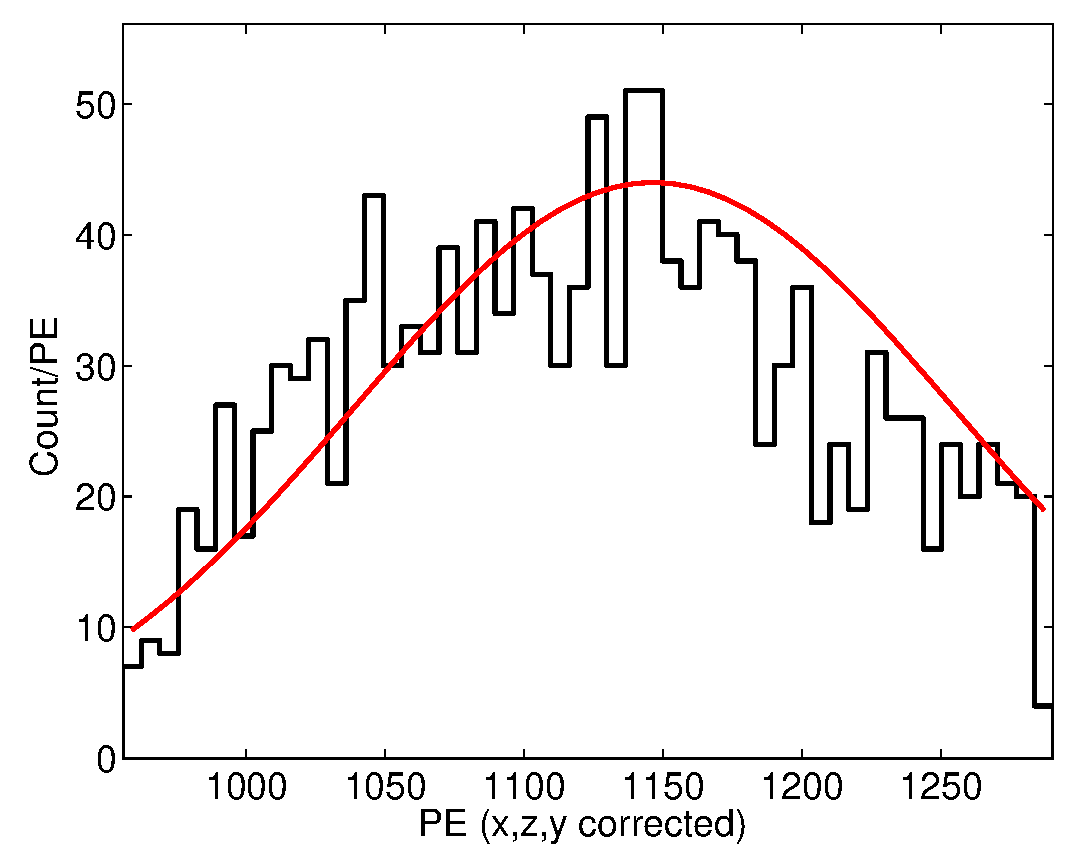
\includegraphics[width=45mm]{Chapter_E_Scale/Figures/Doke_Fits/fit_S1_236.eps}}

\bigskip

\subcaptionbox{\label{fig:1d}}{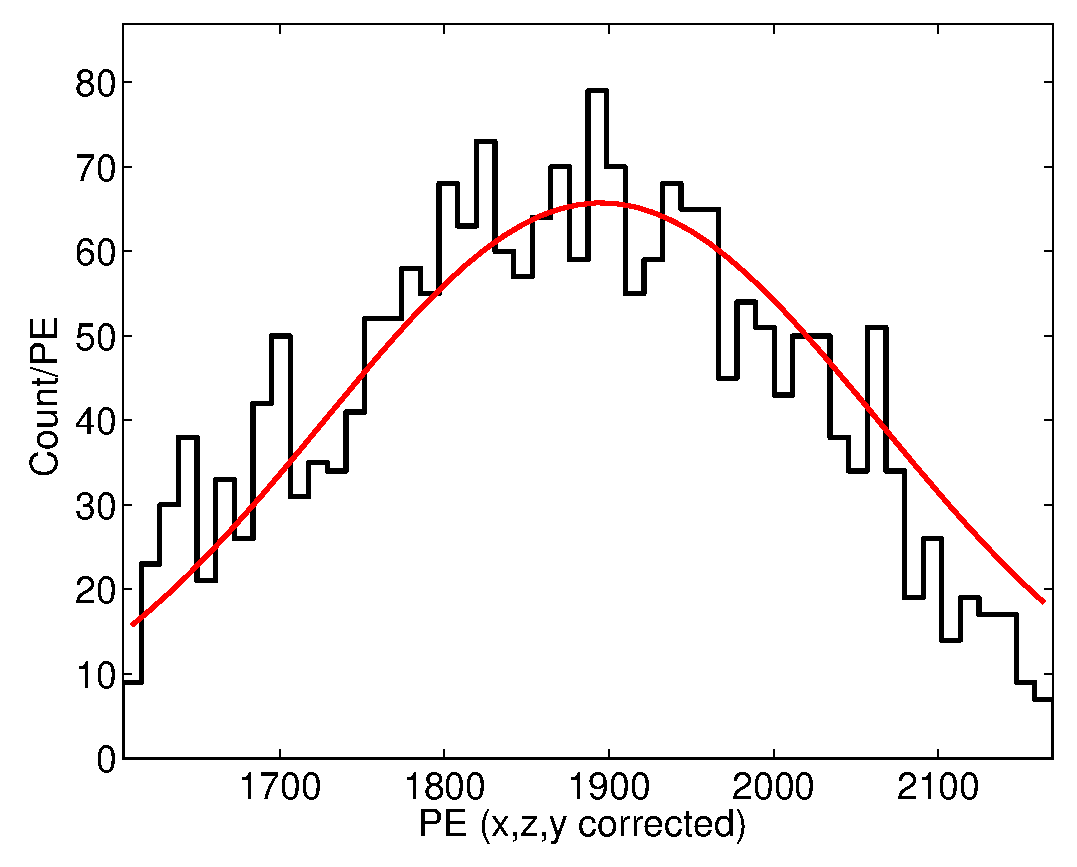
\includegraphics[width=45mm]{Chapter_E_Scale/Figures/Doke_Fits/fit_S1_410.eps}}
\hfill
\subcaptionbox{\label{fig:1e}}{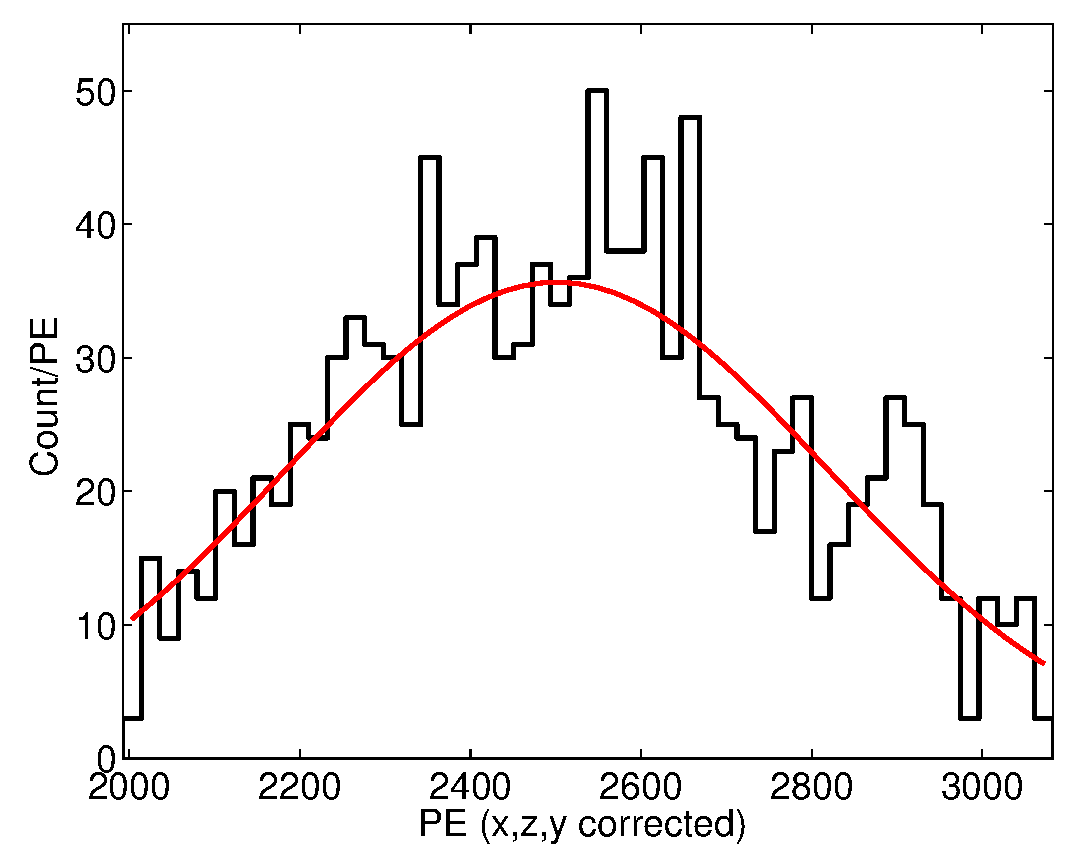
\includegraphics[width=45mm]{Chapter_E_Scale/Figures/Doke_Fits/fit_S1_Bi214.eps}}
\hfill
\subcaptionbox{\label{fig:1f}}{\includegraphics[width=45mm]{Chapter_E_Scale/Figures/Doke_Fits/fit_S1_Cs137.eps}}

\bigskip

\subcaptionbox{\label{fig:1g}}{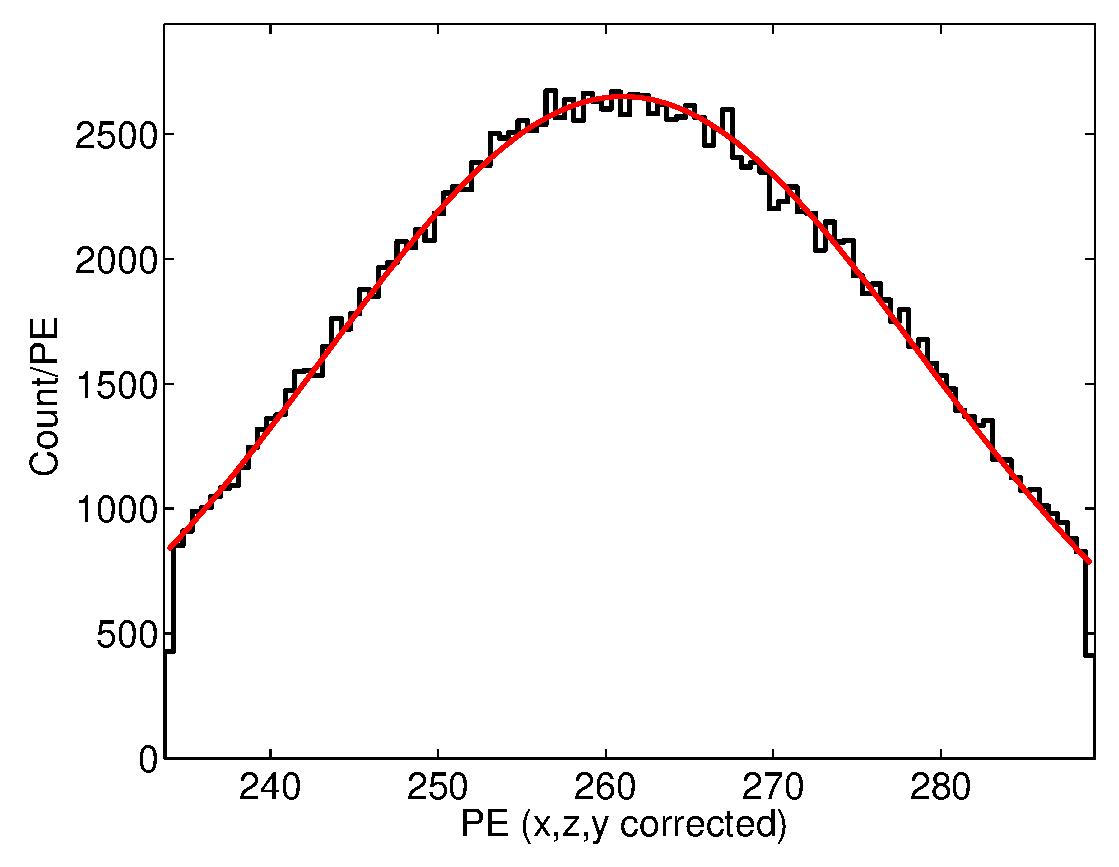
\includegraphics[width=45mm]{Chapter_E_Scale/Figures/Doke_Fits/fit_S1_Kr_50.eps}}
\hfill
\subcaptionbox{\label{fig:1h}}{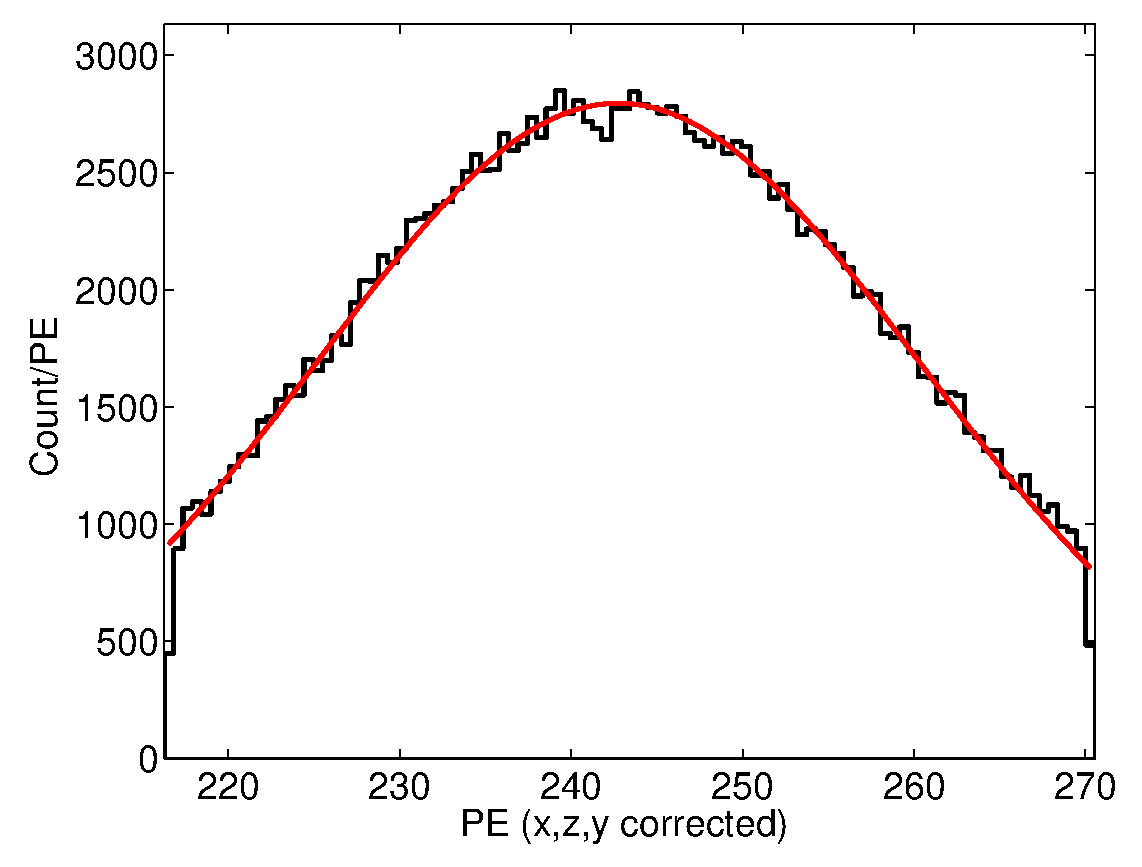
\includegraphics[width=45mm]{Chapter_E_Scale/Figures/Doke_Fits/fit_S1_Kr_100.eps}}
\hfill
\subcaptionbox{\label{fig:1i}}{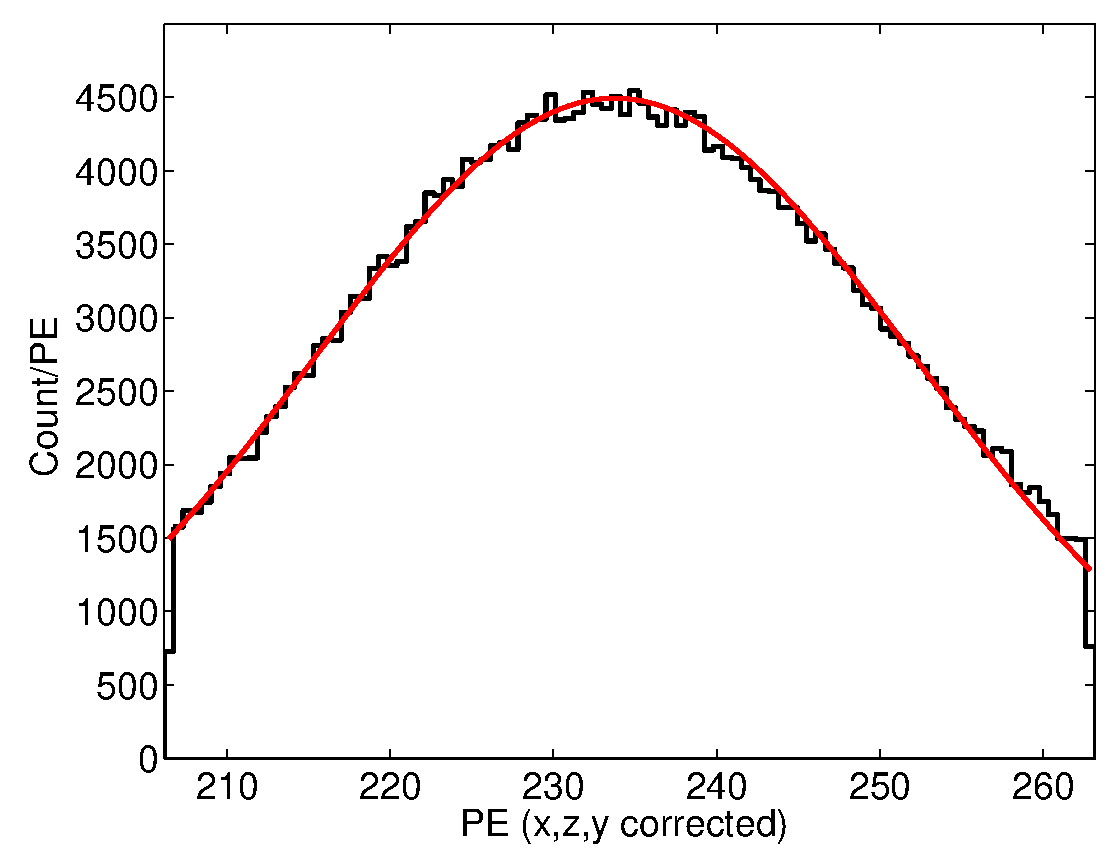
\includegraphics[width=45mm]{Chapter_E_Scale/Figures/Doke_Fits/fit_S1_Kr.eps}}

\caption{S1 fits to sources at nominal field of 170 [V/cm] unless otherwise noted. Source and energy in keV from top left to bottom right: a) $\rm ^{131}Xe$: 163, b) $\rm ^{127}Xe$:  207, c) $\rm ^{127}Xe$ \&  $\rm ^{129m}Xe$: 236.8, d)  $\rm ^{127}Xe$: 410, e) $\rm ^{214}Bi$: 609, f) $\rm ^{137}Cs$: 661.6, g) $\rm ^{83m}Kr$: 41.5 - at 50 [V/cm], h) $\rm ^{83m}Kr$ 41.5 - at 100 [V/cm], i) $\rm ^{83m}Kr$ 41.5 .}
\label{fig:Doke_Fits_S1}
\end{figure}


 \begin{figure}[h!]\centering
 
\subcaptionbox{\label{fig:1a}}{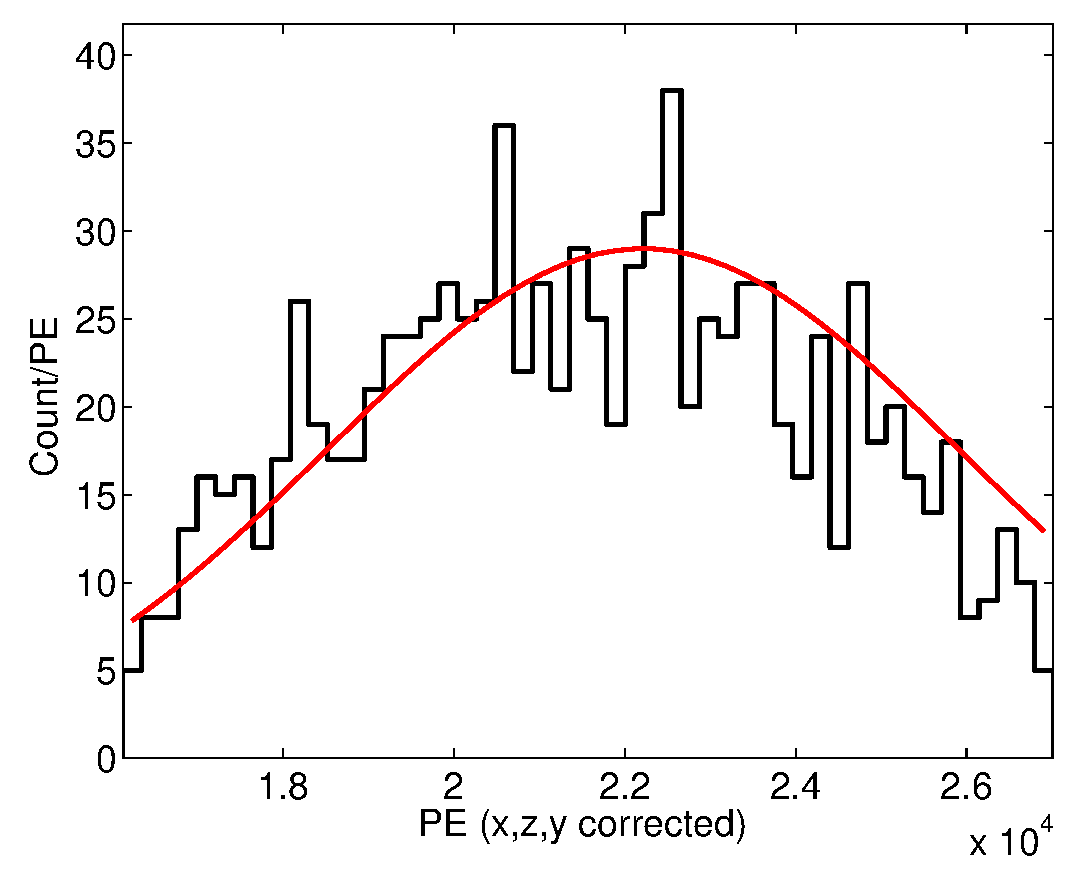
\includegraphics[width=45mm]{Chapter_E_Scale/Figures/Doke_Fits/fit_S2_163.eps}}
\hfill
\subcaptionbox{\label{fig:1b}}{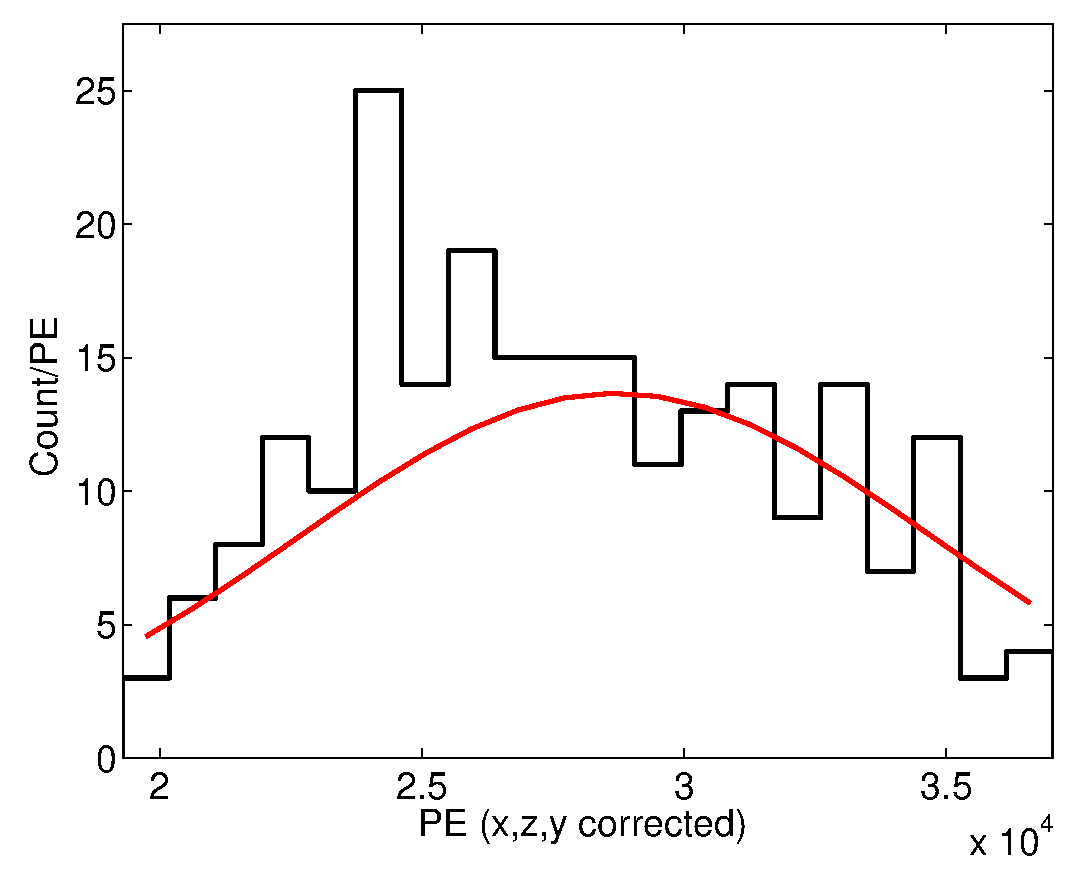
\includegraphics[width=45mm]{Chapter_E_Scale/Figures/Doke_Fits/fit_S2_207.eps}}
\hfill
\subcaptionbox{\label{fig:1c}}{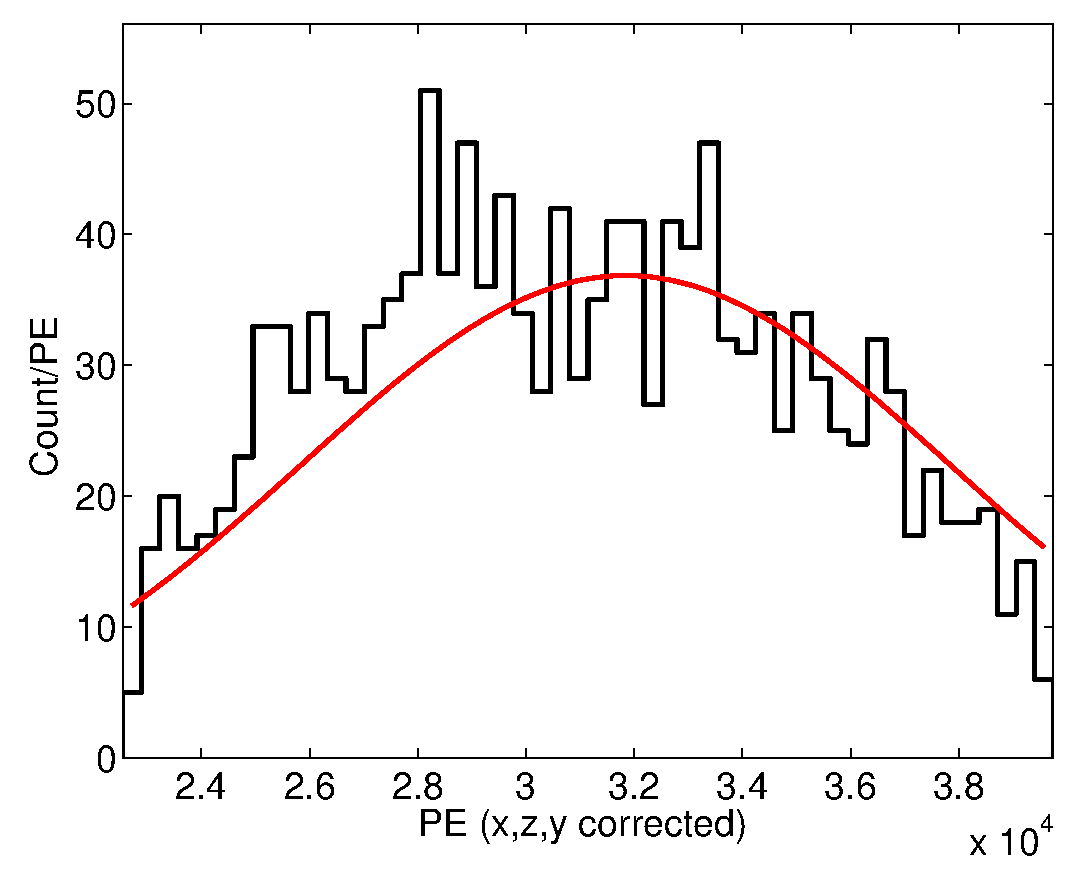
\includegraphics[width=45mm]{Chapter_E_Scale/Figures/Doke_Fits/fit_S2_236.eps}}

\bigskip

\subcaptionbox{\label{fig:1d}}{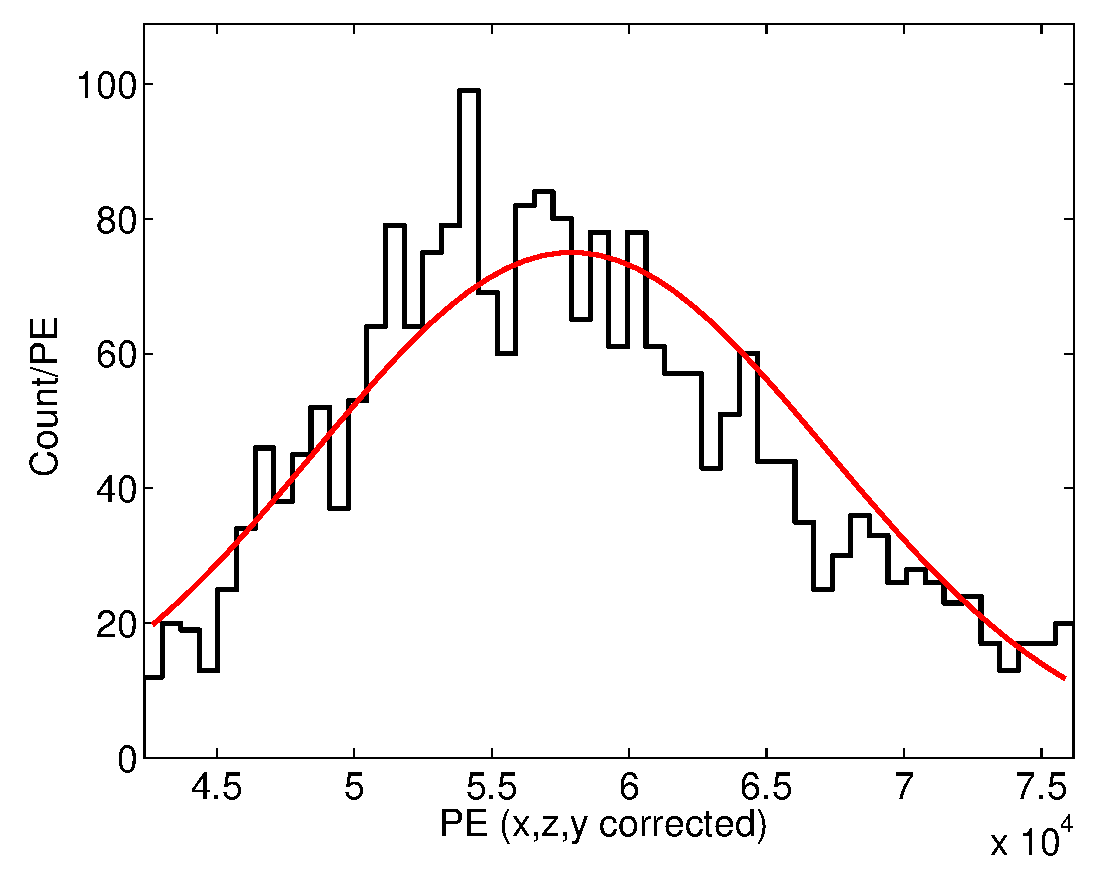
\includegraphics[width=45mm]{Chapter_E_Scale/Figures/Doke_Fits/fit_S2_410.eps}}
\hfill
\subcaptionbox{\label{fig:1e}}{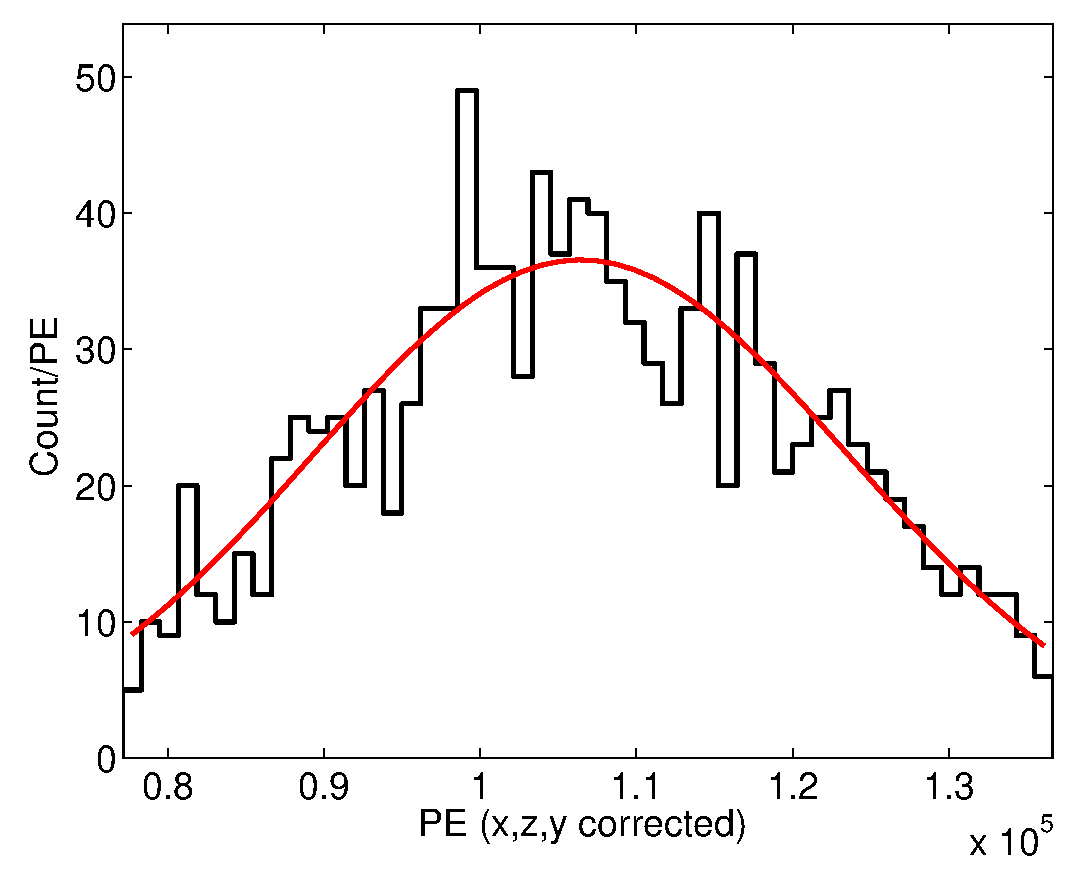
\includegraphics[width=45mm]{Chapter_E_Scale/Figures/Doke_Fits/fit_S2_Bi214.eps}}
\hfill
\subcaptionbox{\label{fig:1f}}{\includegraphics[width=45mm]{Chapter_E_Scale/Figures/Doke_Fits/fit_S2_Cs137.eps}}

\bigskip

\subcaptionbox{\label{fig:1g}}{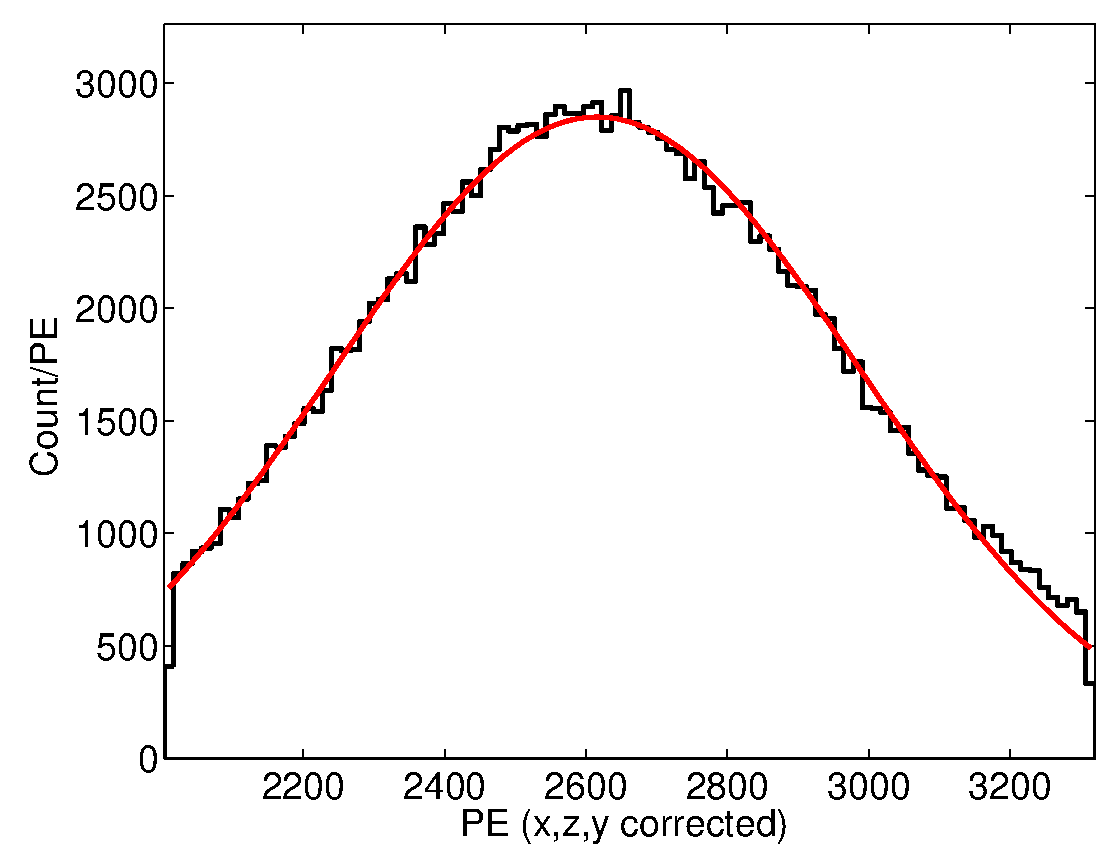
\includegraphics[width=45mm]{Chapter_E_Scale/Figures/Doke_Fits/fit_S2_Kr_50.eps}}
\hfill
\subcaptionbox{\label{fig:1h}}{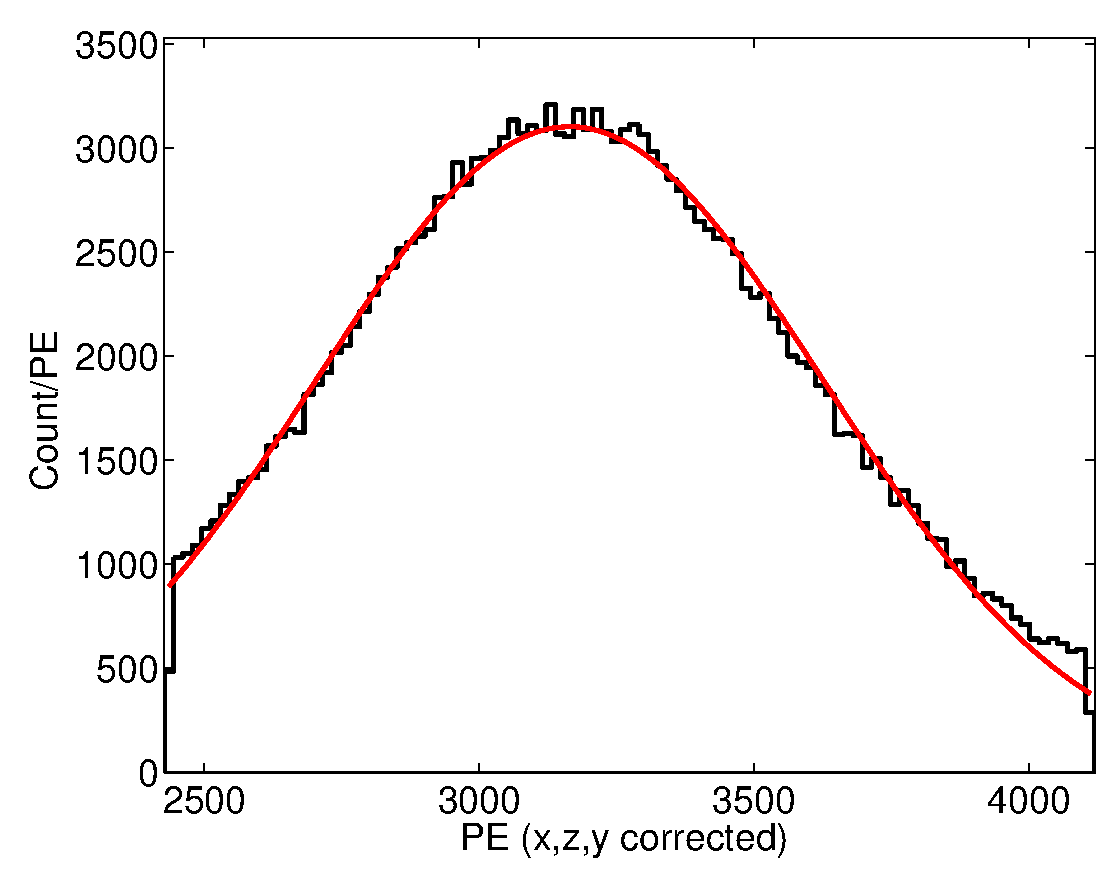
\includegraphics[width=45mm]{Chapter_E_Scale/Figures/Doke_Fits/fit_S2_Kr_100.eps}}
\hfill
\subcaptionbox{\label{fig:1i}}{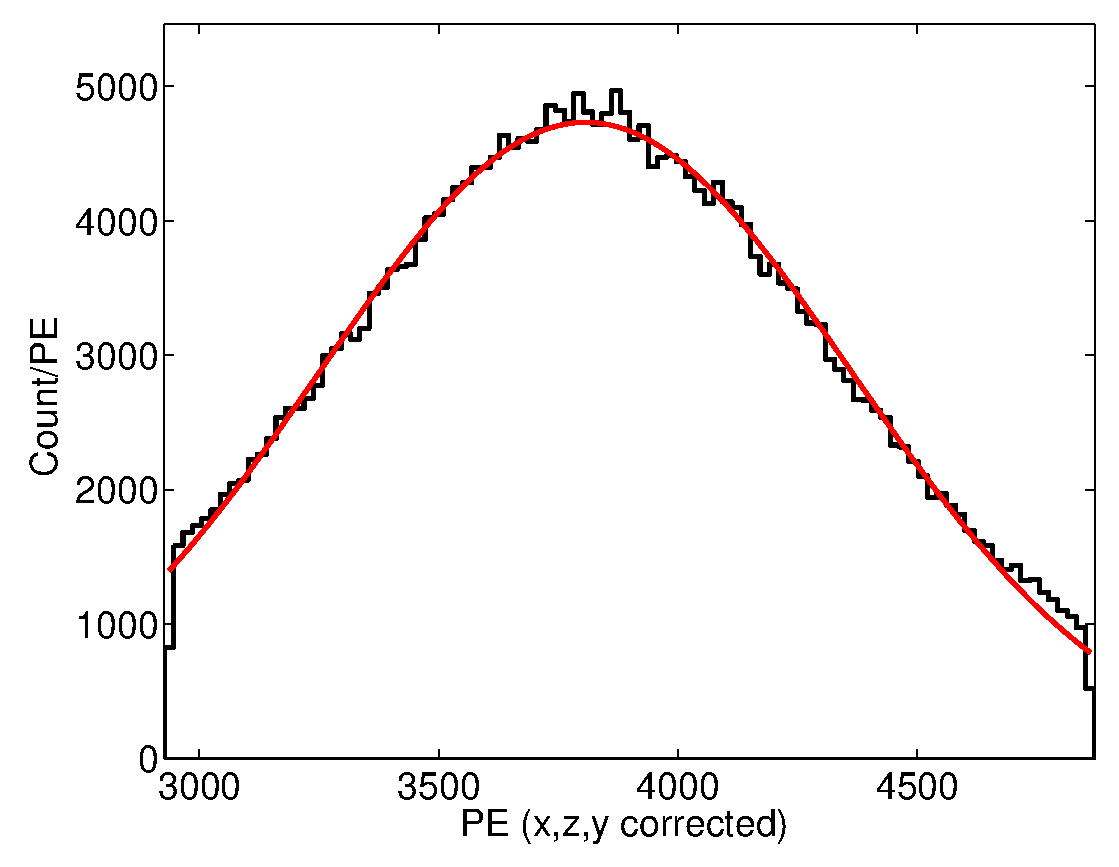
\includegraphics[width=45mm]{Chapter_E_Scale/Figures/Doke_Fits/fit_S2_Kr.eps}}

\caption{S2 fits to sources at nominal field of 170 [V/cm] unless otherwise noted. Source and energy in keV from top left to bottom right: a) $\rm ^{131}Xe$: 163, b) $\rm ^{127}Xe$:  207, c) $\rm ^{127}Xe$ \&  $\rm ^{129m}Xe$: 236.8, d)  $\rm ^{127}Xe$: 410, e) $\rm ^{214}Bi$: 609, f) $\rm ^{137}Cs$: 661.6, g) $\rm ^{83m}Kr$: 41.5 - at 50 [V/cm], h) $\rm ^{83m}Kr$ 41.5 - at 100 [V/cm], i) $\rm ^{83m}Kr$ 41.5 .}
\label{fig:Doke_Fits_S2}
\end{figure}



Figure \ref{fig:Doke_E} is the final Doke plot for multiple peaks the theory describes the data well using the optimal fit for g1 and g2, for each increase in number of photons there is a corresponding decrease in the number of electrons and visa versa. The relatively large error on g2 is due to the distance of the data points from the x-intercept. As stated before the values of g1 and g2 can be locally degenerate as long as their ratio remains a constant. Thus for future studies it will be important to probe more of the parameter space in order to place a tighter constraint on gains g1 and g2.


 \begin{figure}[h!]\centering
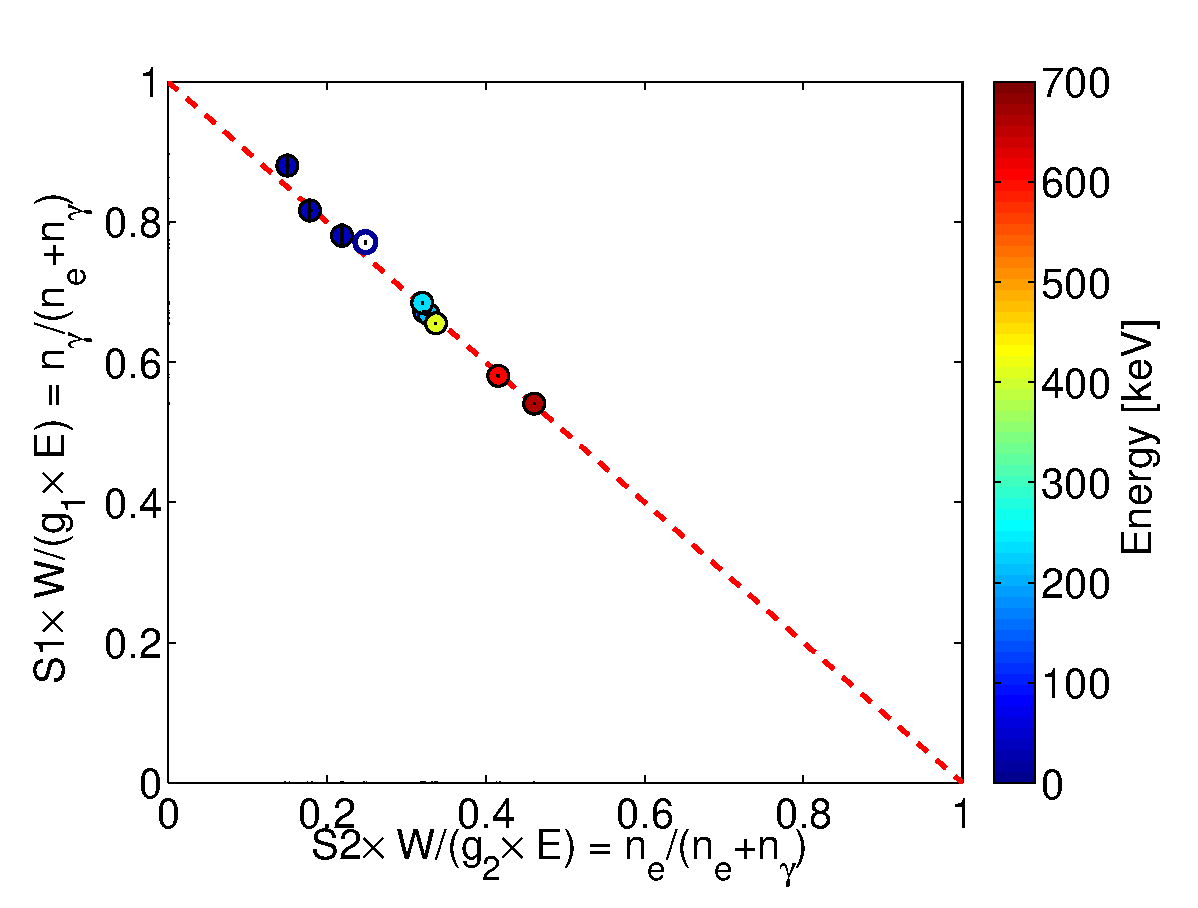
\includegraphics[width=100mm]{Chapter_E_Scale/Figures/S1S2_Doke2_3.eps}
\caption{Doke plot of the data showing the light yield vs. charge yield. Only solid circles are used for the fit, the open circle is the Xe K shell X-ray from the detector edge.}
\label{fig:Doke_E}
\end{figure}

\newpage

\section{Finding Errors with MCMC}
\label{sec:MCMC}
The error bars reported in this section on g1 and g2 are from the error in the slope and intercept of the linear fit in the Doke plot derived using MCMC. For calculating the error in slope and intercept  three random walkers were used at each data point and allowed to take 500 steps.The MCMC takes into account the covariance of the parameters, shown in figure \ref{fig:MCMC} as a two dimensional Gaussian. There is a strong negative correlation between the slope m and intercept b which is the result of the degeneracy between gains g1 and g2 used to reconstruct energy by combining the light and charge signal. Thus, the error on g1 and g2 is such that for the positive maxima deviation in g1 we reach the negative maxima of the error on g2, and visa versa. Using standard reduced $\chi^2$ for fitting and calculating errors in the slope and intercept would be underestimated the true error by a factor of five as it does not account for the degeneracy of the anti-correlated gains. 



\begin{figure}[h!]\centering
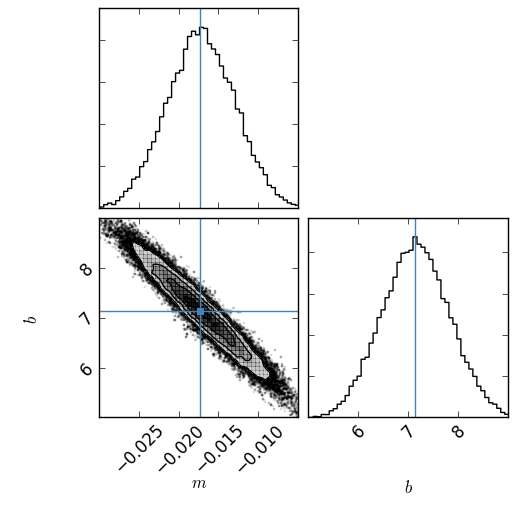
\includegraphics[width=100mm]{Chapter_E_Scale/Figures/MCMC/triangle.png} % also line-time.png
\caption{MCMC for the linear fit to the Doke plot. There is a strong negative correlation between the slope m and intercept b which results from the degeneracy between gains g1 and g2. }
\label{fig:MCMC} 
\end{figure}

\newpage

\section{Combined Energy Space}

With the values of g1 and g2 known the combined energy of events can be reconstructed with a significant improvement over using only the light or charge channel. In combined energy space recombination fluctuations are removed by the anti correlation of light and charge production and any residual smearing is due to intrinsic detector resolution (discussed later in section :) . Figure \ref{fig:CE_hist} shows the energy histograms of the data used for the fits to gains g1 and g2 including the xenon activation lines and the $\rm^{137}Cs$ calibration, along with a zoom in of the xenon K shell Xray at 34 keV. With the energy scale calibrated we can now reconstruct the energy of the events and convert the measured S1 and S2 signals to fundamental quanta using  the gains g1,g2 allowing us to untangle instrumental and recombination fluctuations and measure light and charge yields.


\begin{figure}[h!]\centering
 
\subcaptionbox{\label{fig:1a}}{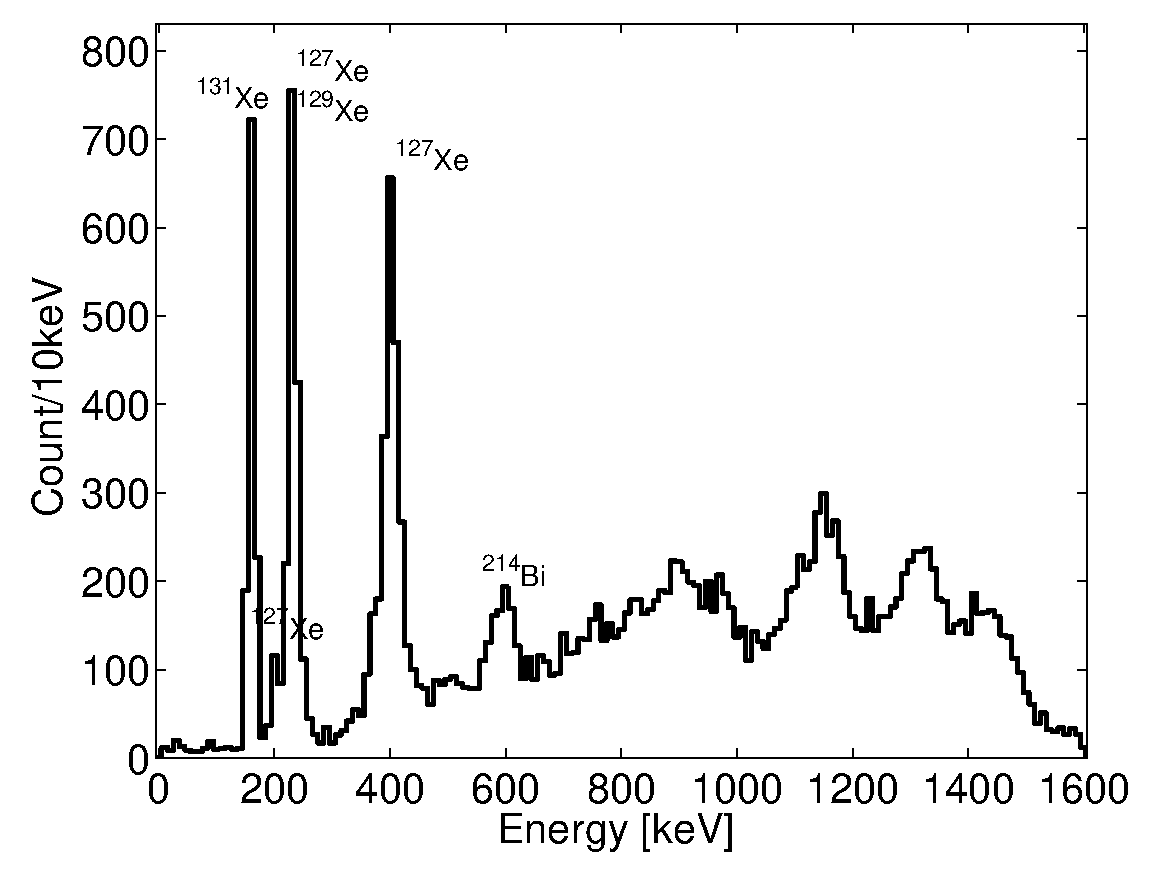
\includegraphics[width=70mm]{Chapter_E_Scale/Figures/Combined_E/Xe_act_E.eps}}
\hfill
\subcaptionbox{\label{fig:1b}}{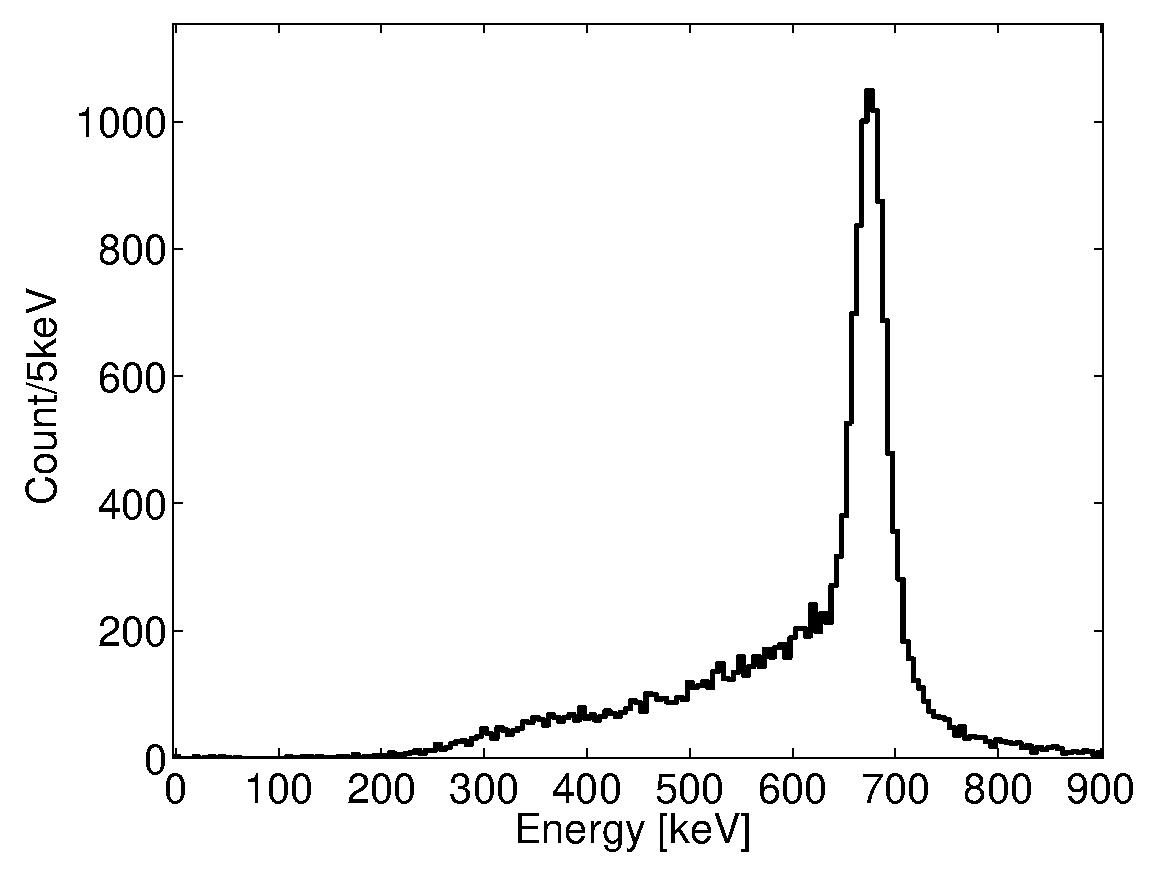
\includegraphics[width=70mm]{Chapter_E_Scale/Figures/Combined_E/Cs_E.eps}}


\bigskip

\subcaptionbox{\label{fig:1c}}{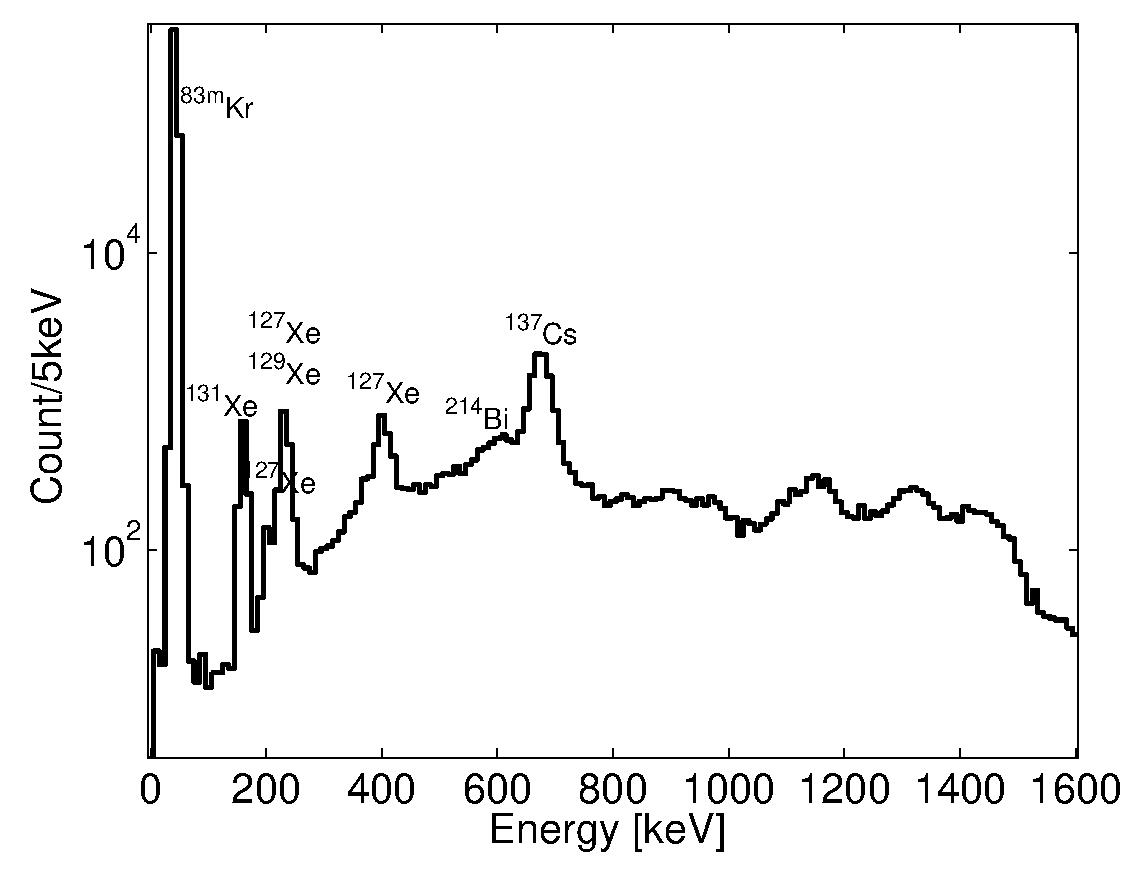
\includegraphics[width=70mm]{Chapter_E_Scale/Figures/Combined_E/Cs_Kr_Xe_E.eps}}
\hfill
\subcaptionbox{\label{fig:1d}}{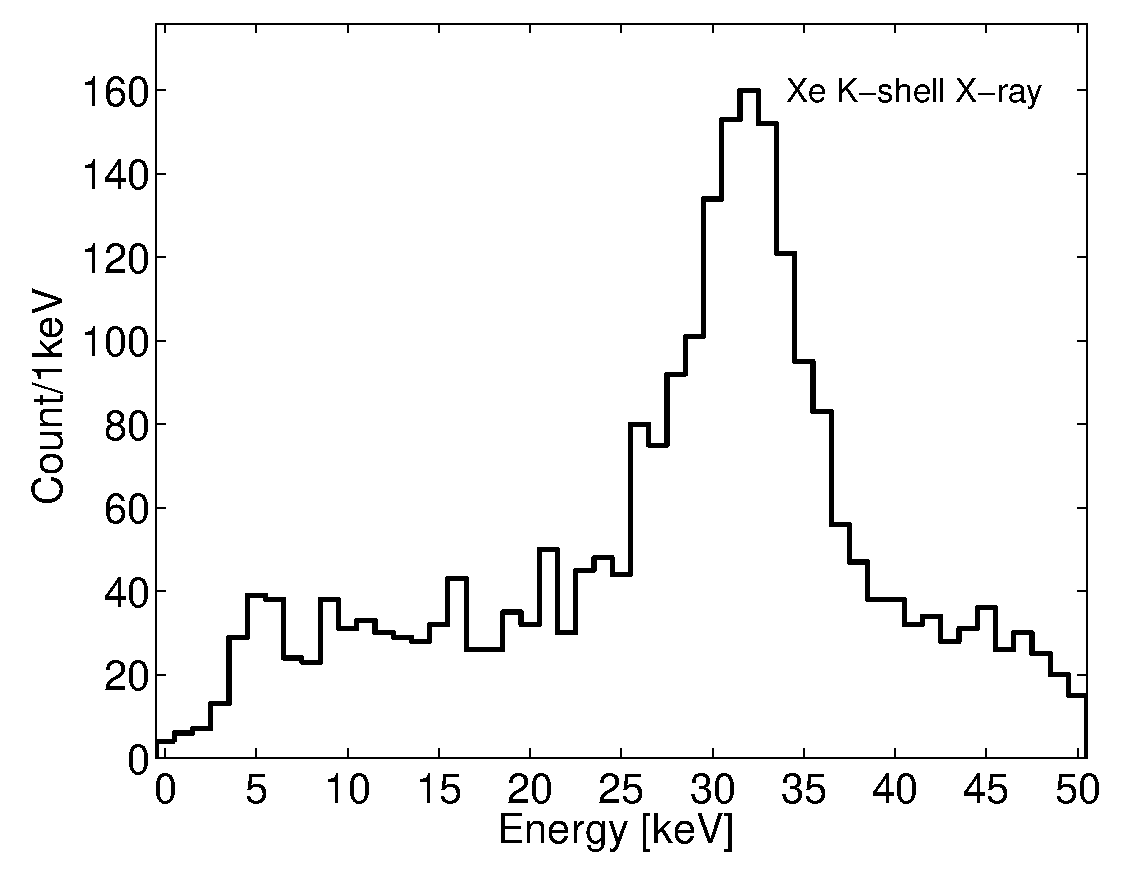
\includegraphics[width=70mm]{Chapter_E_Scale/Figures/Combined_E/X-ray_Xe_E.eps}}


\caption{Combined energy scale. a) The xenon activation lines from early in the run. b) $\rm^{137}Cs$ calibration data. c) All calibration data including the $\rm^{83m}Kr$ calibration. d) Xenon X-ray.}
\label{fig:CE_hist}
\end{figure}



\section{Light Collection and Electron extraction}

The value of g1 represents the mean efficiency for collecting photons at the center of the LUX detector, the response to S1 light is flat fielded and normalized to the detector center (section Kr calibrations). The measured value of g1= $\rm0.097\pm0.008$ implies a 9.7\% probability of a photon propagated from the center of the detector stricking a PMT and being converting into a photo electron (PE) signal. The value of g2 represents the average number of PE collected for each electron that escaped recombination at the initial interaction site and then drifted,by the electric field, towards liquid-gas interface where it is extracted with some probability $\rm \epsilon$. The value of g2 can be thought of as the average single electron size in PE times the extraction probability $\rm \epsilon$.
\begin{equation}
\rm g2=\epsilon \times SE
\end{equation}
 
 \noindent where S2 is the average pulse area of a single electron. The S2 signals are corrected for depth as impurities exponentially attenuate electrons drifting through the xenon, section \ref{Ch:3}. The LUX detector is low enough in threshold to observe singe electrons being extracted from the liquid. Comparing the value of g2 derived from the Doke method with the single electron size is a good sanity check on the energy scale calibration. As the electrons are extracted from the liquid they are accelerated by larger field between the gate and anode where they electo-lumanesance, a single extracted electron creates tens to hundreds of photons which are collected by both PMT arrays. We can cut on the single electron population (small S2 pulses without an associated S1) and measure the single electron size along with the extraction efficiency efficiency. The extraction efficiency is defined as the probability that an electron will be extracted from the liquid into the gas in a region, held at 3.5 kV in the liquid between the anode and the gate. For a given event the extraction of electrons is a binomial processes with a rate approaching unity for fields above 5 kV \cite{Recomb_Time_Extraction} \cite{Aprile_LXe_overview}. Figure \ref{fig:SingleE}, shows the single electron size as measured by the bottom PMT array (used for S2 pulses in the LUX detector to avoid saturation). The population is modeled by a skew Gaussian due to the Poisson nature of measuring only a handful of photo electrons (PE) per extracted electron. The mean of the distribution is found to be 9.7 PE/$\rm e^-$ with a width of $\rm \sigma SE$= 3.6 Phe/$\rm e^-$. Thus, the extraction efficiency is g2 over the single electron size and is found to be (59.3$\rm \pm$14)\%, given the extraction field the value is in good agreement with previous measurements in other xenon detectors \cite{Recomb_Time_Extraction} \cite{Aprile_LXe_overview}.

\begin{figure}[h!]\centering
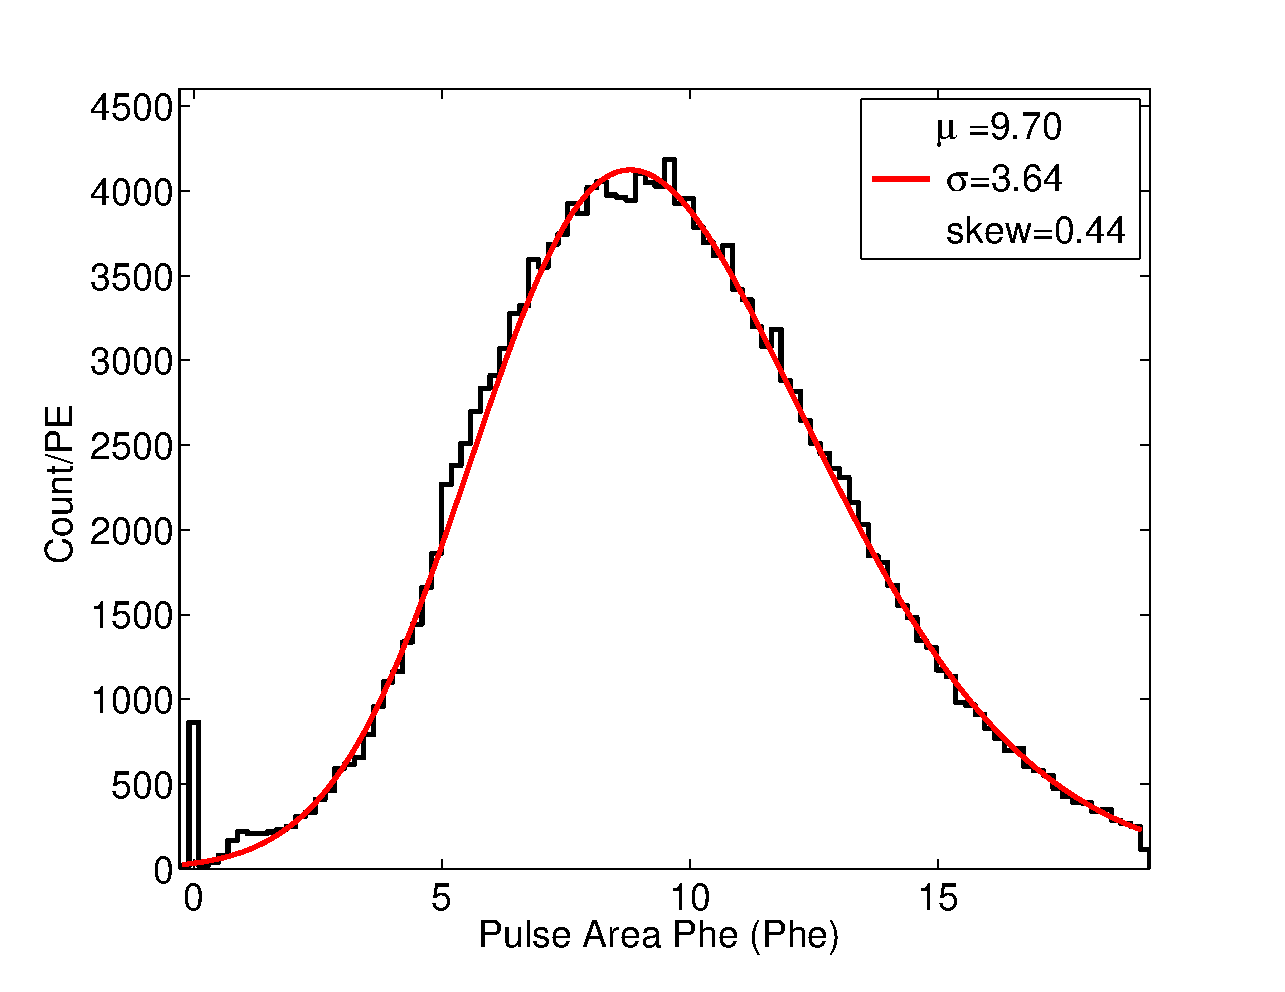
\includegraphics[width=100mm]{Chapter_E_Scale/Figures/bottom_SE.eps}
\caption{Single electron distribution as seen by the bottom PMT array fitted with a skew Gaussian model to account for the underling Poisson statistics of observing between 9 and 10 photo electrons (PE) for each electron leaving the liquid and entering to the gas phase at a higher field causing electro-luminescence. The $\rm \mu$ of the fit represents the true mean of the skew Gaussian distribution. }
\label{fig:SingleE}
\end{figure}

\newpage

\section{Tritium Beta Spectrum}

The energy calibration in the WIMP search region can be tested by using the tritium calibration source described in Chapter[]. Tritium has a Q value of 18.6 keV \cite{Tritium_Q}, a mean beta energy of 5.6 keV \cite{Tritium_Mean} and a mode of 3.4 keV \cite{Tritium_Eq} making it ideal for calibrating the LUX detector at the lowest energies. The tritium beta spectrum produces events at energies well below the detector threshold. Therefore, by comparing the reconstructed energy to the true tritium beta spectrum we can extract the energy threshold. We account for the detector resolution, smearing, by applying the empirically determined resolution measured in Chapter []. Smearing the spectrum with the empirically determined detector resolution is in good agreement with that expected from the simulation package of LUXSIM.

Figure \ref{fig:E_spec} (a,b) shows the reconstructed energy from a tritium calibration at the default filed setting of 170 V/cm. The calibration contains 140,000 tritium events with an expected 2$\pm$1 background events in black. In red, a simulated tritium beta spectrum from the LUXSIM package with modeled detector resolution and having gone through data processing framework.  In blue and green are the theoretical tritium beta spectrum with infinite detector resolution and with the added resolution of the LUX detector, respectively.  Figure \ref{fig:E_spec} (c,d) shows the same calibration but at a lower drift field setting of 100 V/cm with only 4,500 tritium events and an expected 1$\pm$ background events.

\newpage

\begin{figure}[h!]\centering
 
\subcaptionbox{170 V/cm \label{fig:3a}}{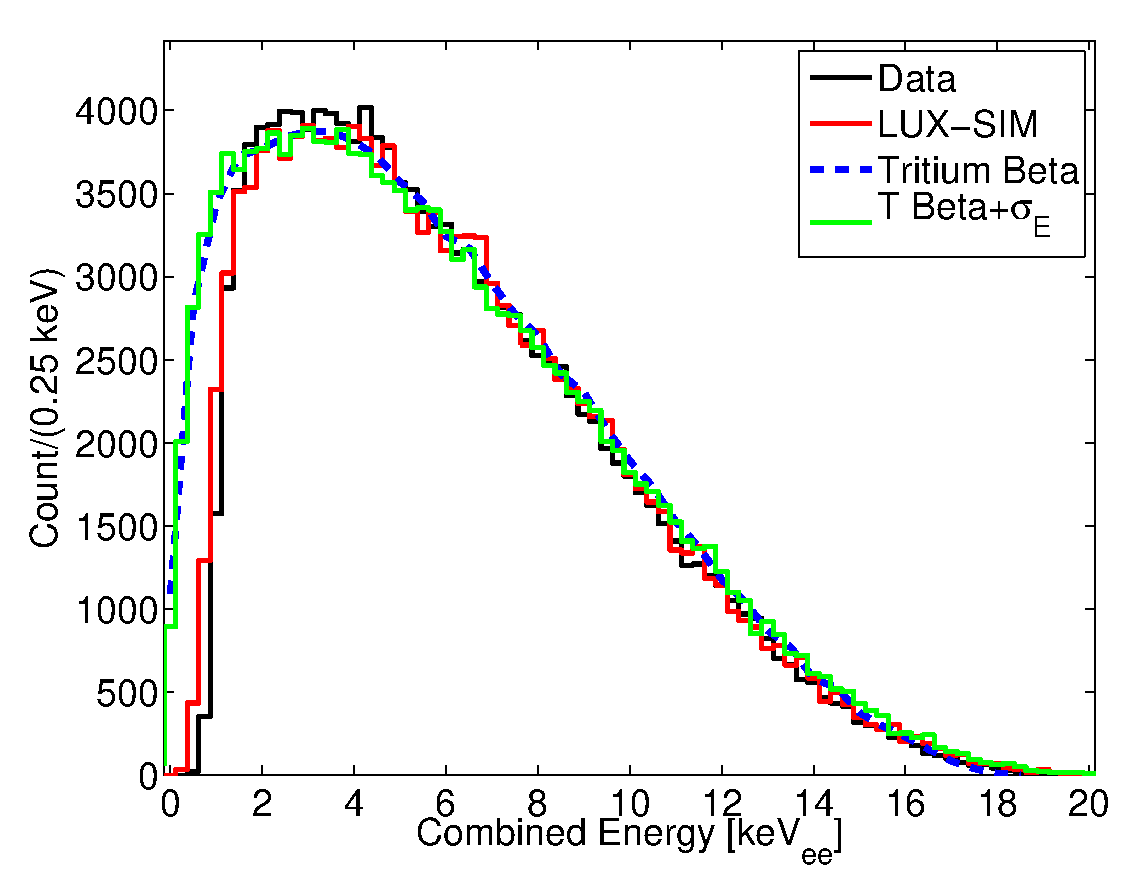
\includegraphics[width=73mm]{Chapter_E_Scale/Figures/E_Spec/E_spec_compare_SIM.eps}}
\hfill
\subcaptionbox{170 V/cm \label{fig:3b}}{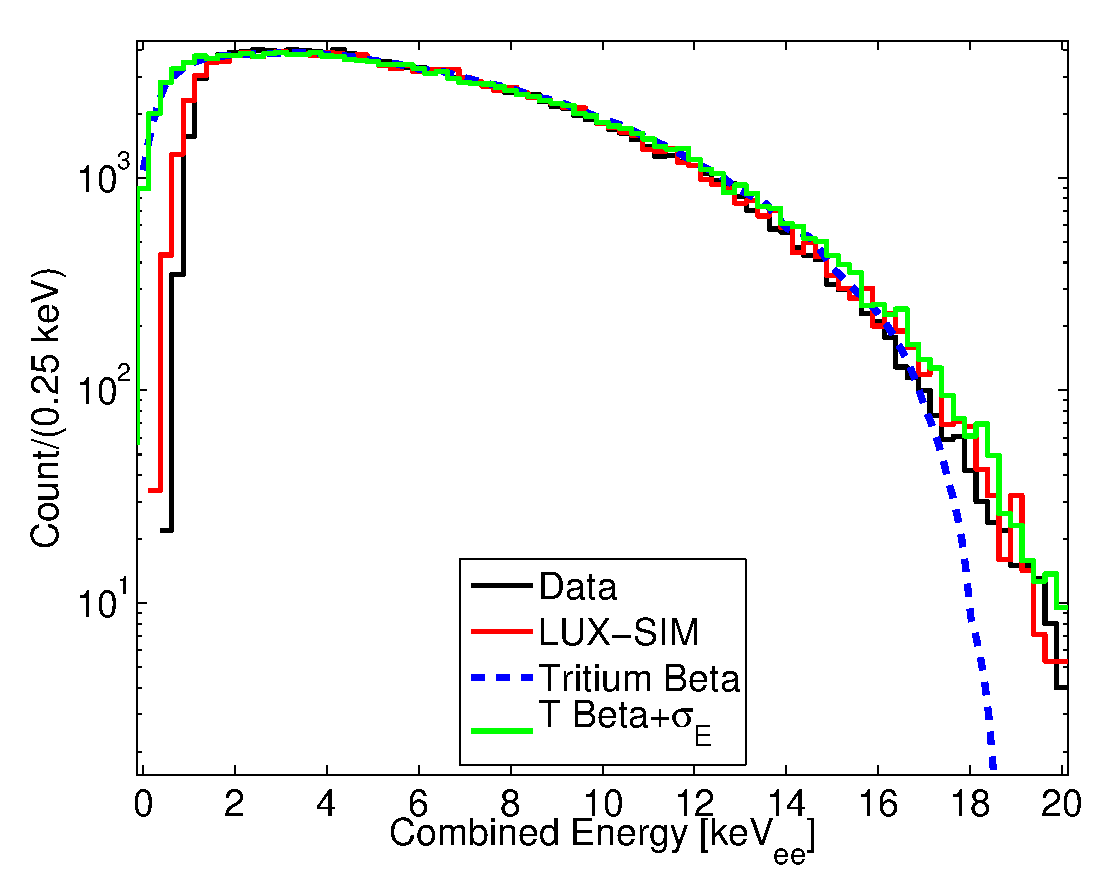
\includegraphics[width=73mm]{Chapter_E_Scale/Figures/E_Spec/E_spec_compare_SIM_log_.eps}}

\bigskip

\subcaptionbox{100 V/cm \label{fig:3c}}{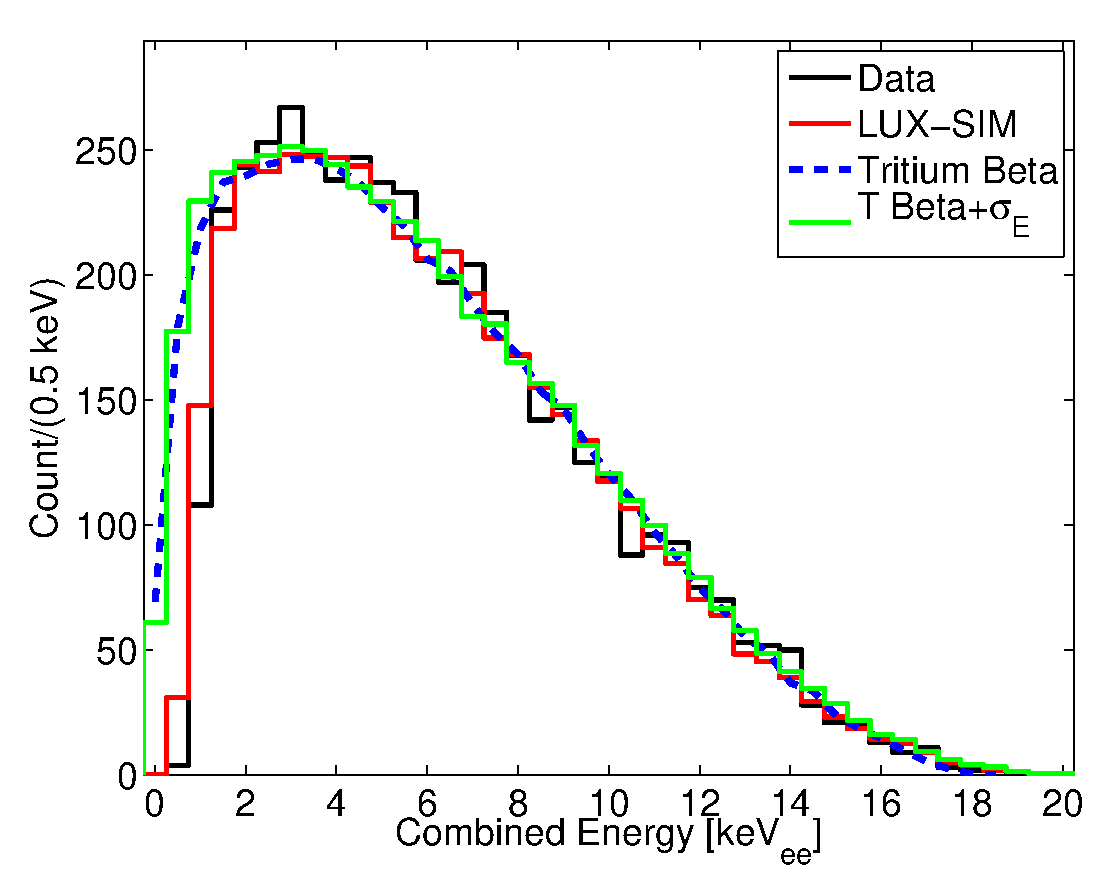
\includegraphics[width=73mm]{Chapter_E_Scale/Figures/Spec_Thresh_100/E_spec_compare_SIM.eps}}
\hfill
\subcaptionbox{100 V/cm \label{fig:3c}}{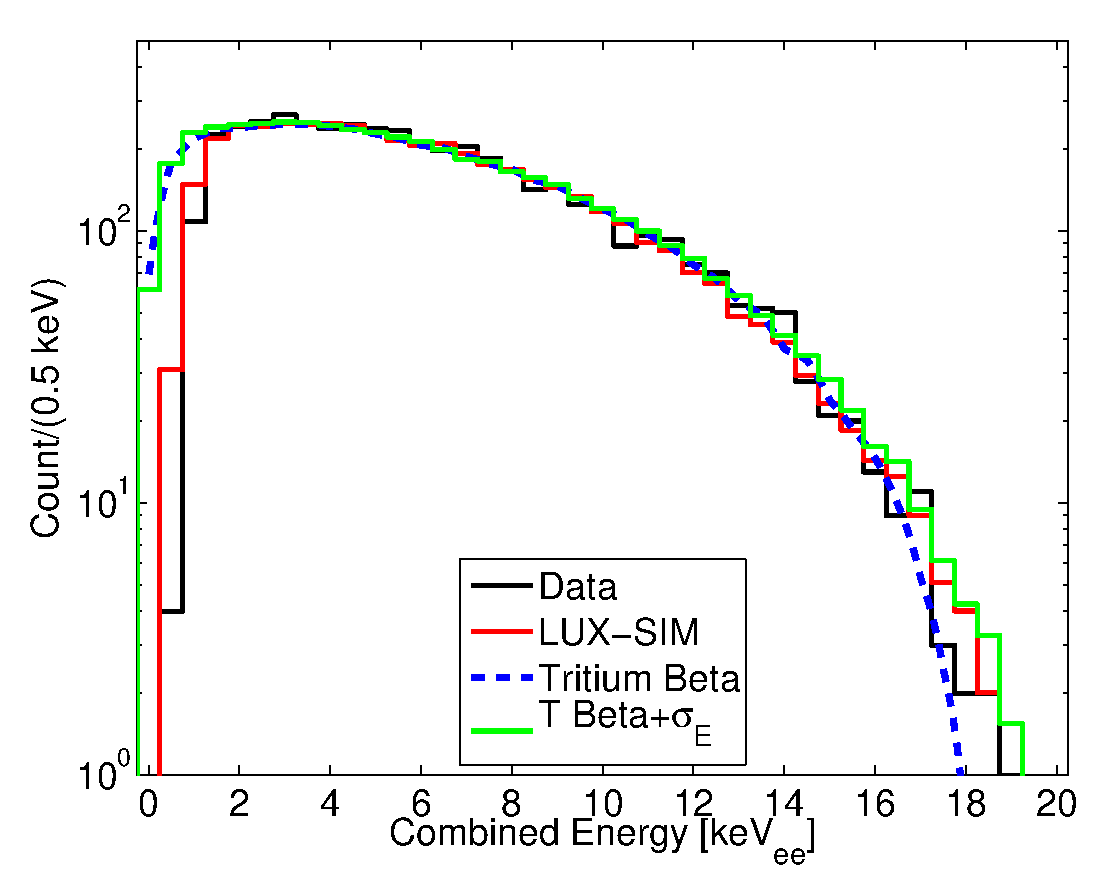
\includegraphics[width=73mm]{Chapter_E_Scale/Figures/Spec_Thresh_100/E_spec_compare_SIM_log_.eps}}

\caption{The tritium energy spectrum reconstructed from the data (black). Along with LUX SIM (blue), and the true tritium beta spectrum (blue) and a tritium spectrum smeared with detector resolution (green). }
\label{fig:E_spec}
\end{figure}

The reconstructed energy spectrum is in good agreement with the expected tritium beta spectrum with detector resolution, using both LUXSIM and the empirically determined resolution. The detector threshold reaches 100\% at about 1.5 keV making the tritium beta peak clearly visible providing crucial cross check of the reconstructed energy around the WIMP search region of interest (1-5 keV). The 18.6 keV endpoint is another good low energy calibration point. We find that the end point of the reconstructed energy spectrum is consistent with that expected when convolving the true tritium beta spectrum with detector resolution, visible in log space. Though the energy scale for ER events was events was calibrated using mono energetic sources well above the tritium Q value the reconstructed tritium beta spectrum lines up with the expectation all the way down to the 1.5 keV threshold.


Figure \ref{fig:Thres} and \ref{fig:Thres_100} show the S1,S2 and Energy threshold attained by comparing the data to the expected photon, electron and energy spectrum, at 170 and 100 V/cm. The energy threshold is set by the light collection of the much smaller S1 signal. For the energy threshold we find roughly 50\% efficiency at 1 $\rm keV_{ee}$ approaching 100\% at 1.5 $\rm keV_{ee}$ regardless of the applied field. The S1 threshold is 50\% at 2 PE and surpassed 90\% above 3 PE. This translates to an $\rm S2_b$ threshold for golden events of 50\% at 300 PE approaching 100\% a 400 PE. Extracting the threshold will be discussed in further detail in Section ... .


\begin{figure}[h!]\centering
 
\subcaptionbox{S1 \label{fig:3a}}{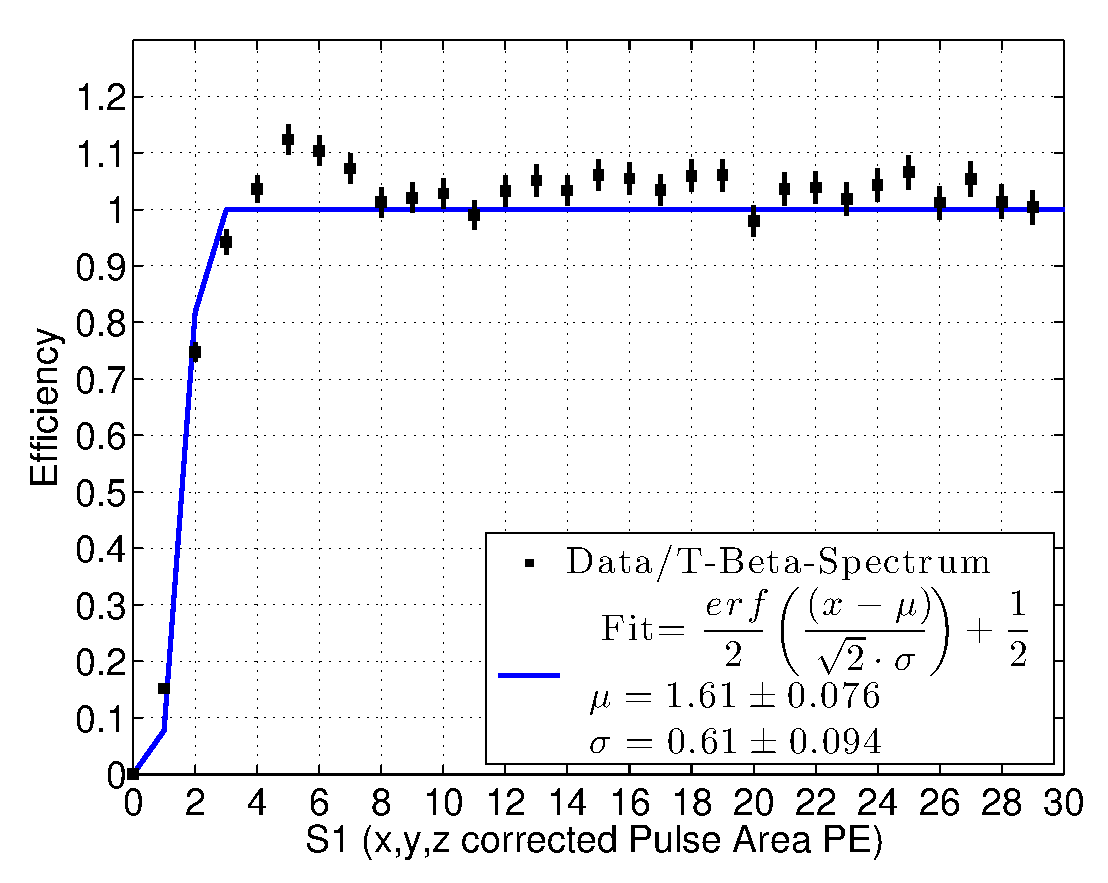
\includegraphics[width=73mm]{Chapter_E_Scale/Figures/S1S2_Spectra/S1_Thres_.eps}}
\hfill
\subcaptionbox{$\rm S2_b$ (golden) \label{fig:3b}}{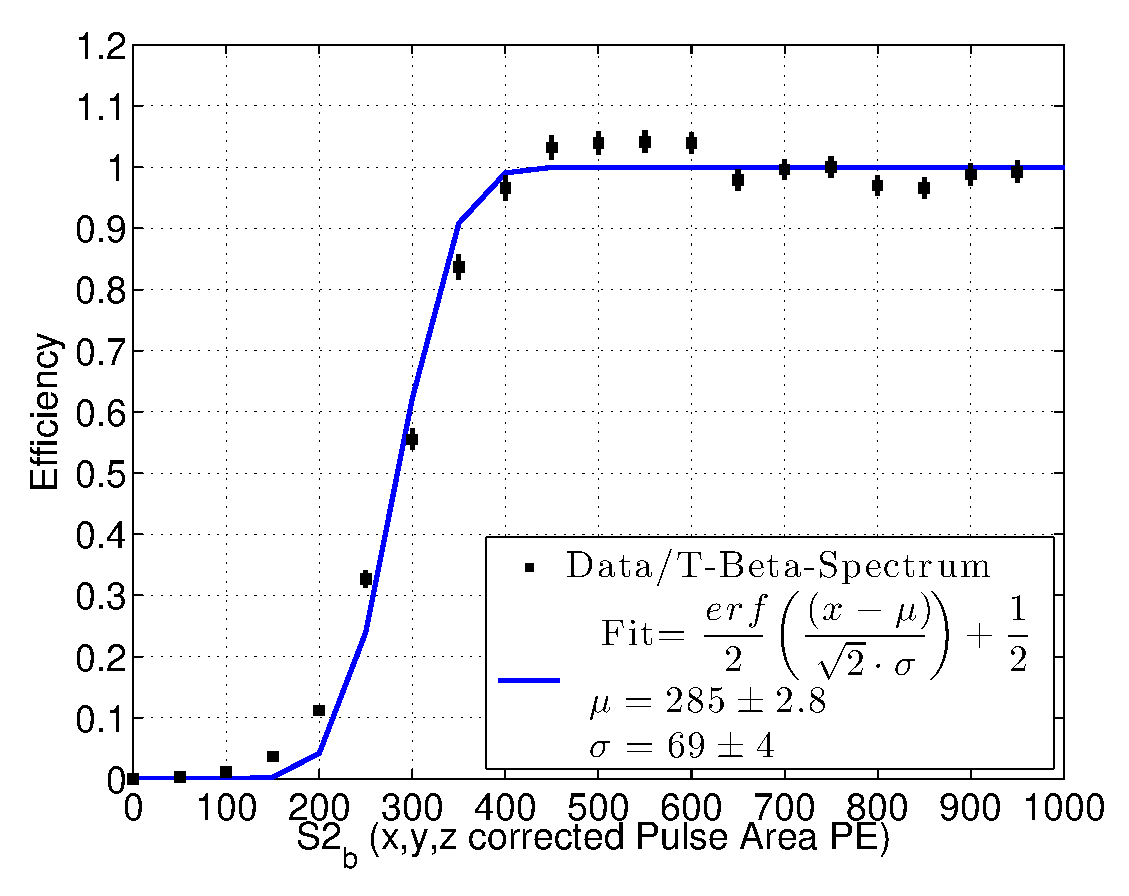
\includegraphics[width=73mm]{Chapter_E_Scale/Figures/S1S2_Spectra/S2_Thres_.eps}}

\bigskip

\subcaptionbox{Combined Energy \label{fig:3c}}{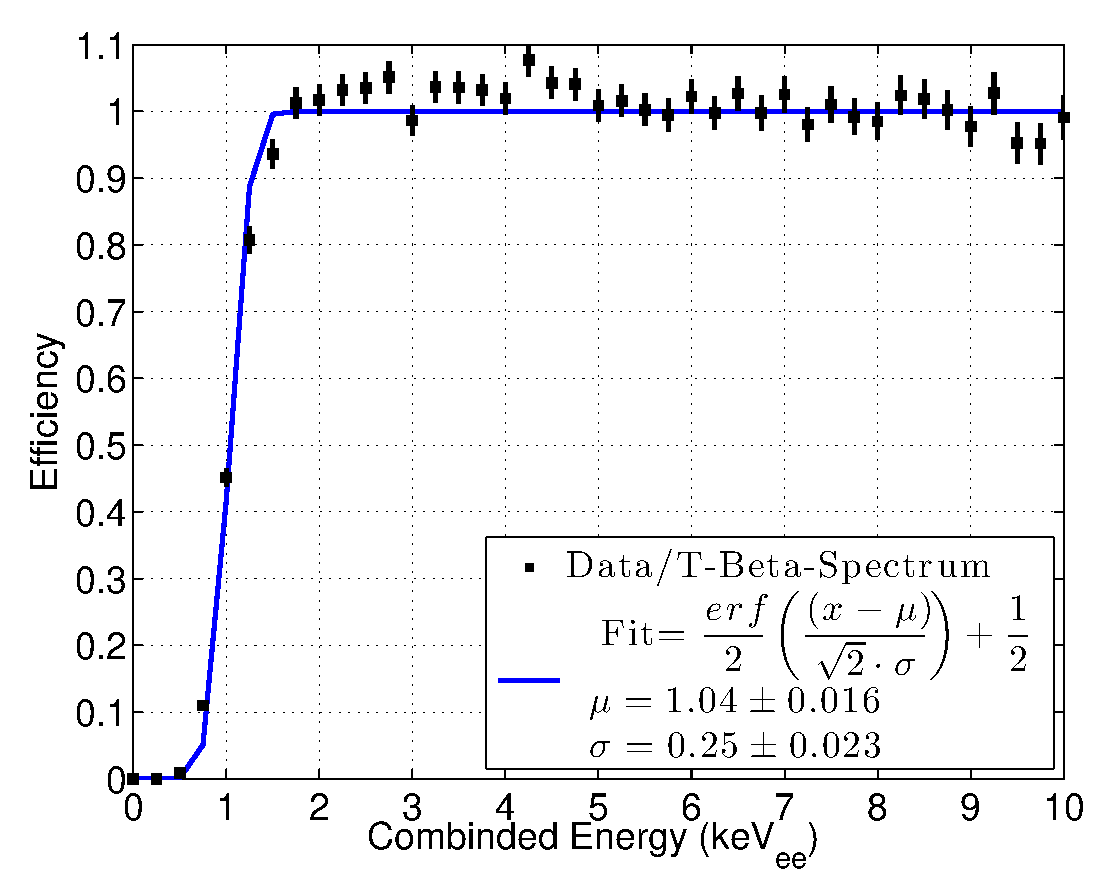
\includegraphics[width=73mm]{Chapter_E_Scale/Figures/E_Spec/E_Thres_LY_QY_iter1.eps}}

\caption{Threshold calculated from difference of simulated Tritium S1, S2 and energy spectra at 170 V/cm. a) S1 b) $\rm S2_b$, c) Combined Energy .}
\label{fig:Thres}
\end{figure}


\begin{figure}[h!]\centering
 
\subcaptionbox{S1 \label{fig:3a}}{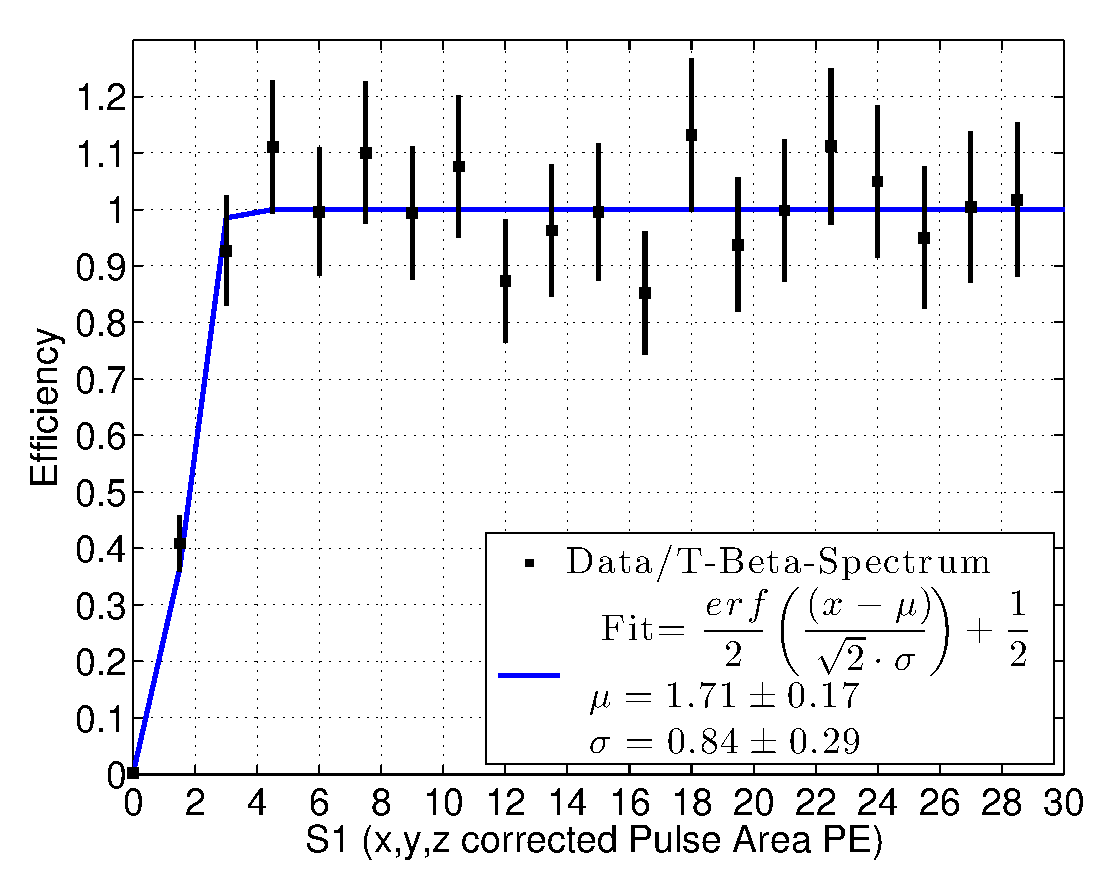
\includegraphics[width=73mm]{Chapter_E_Scale/Figures/Spec_Thresh_100/S1_Thres_.eps}}
\hfill
\subcaptionbox{$\rm S2_b$ (golden) \label{fig:3b}}{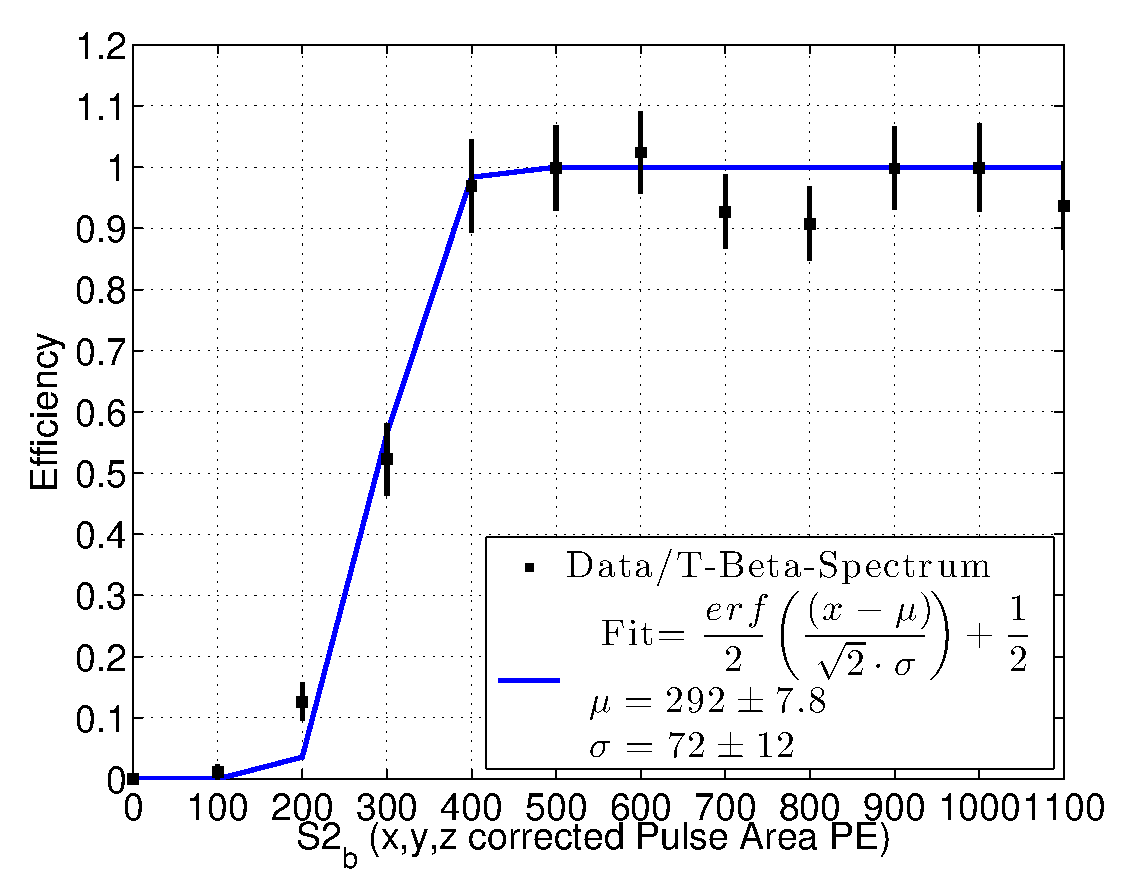
\includegraphics[width=73mm]{Chapter_E_Scale/Figures/Spec_Thresh_100/S2_Thres_.eps}}

\bigskip

\subcaptionbox{Combined Energy \label{fig:3c}}{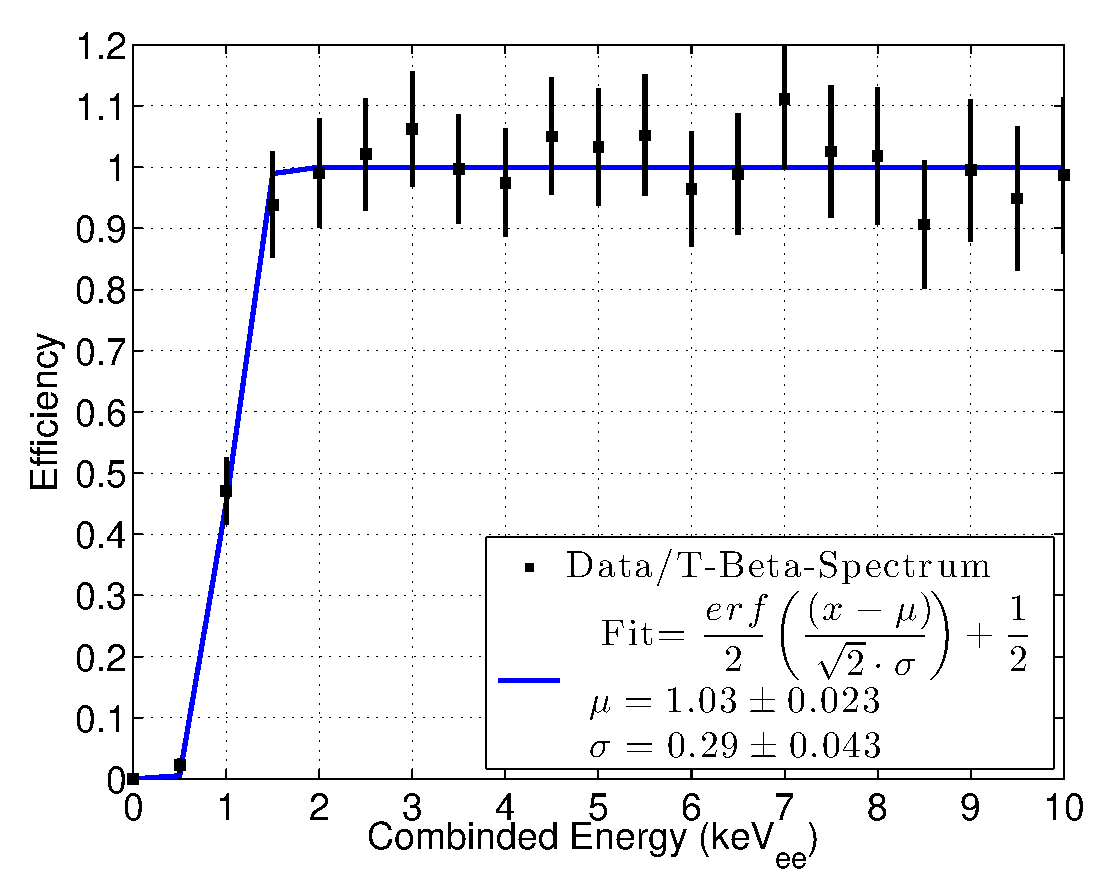
\includegraphics[width=73mm]{Chapter_E_Scale/Figures/Spec_Thresh_100/E_Thres_.eps}}

\caption{Threshold calculated from difference of simulated Tritium S1, S2 and energy spectra at 100 V/cm. a) S1 b) $\rm S2_b$, c) Combined Energy .}
\label{fig:Thres_100}
\end{figure}